\documentclass[a4paper,fontsize=12pt,toc=bib,halfparskip]{scrartcl}

\usepackage[utf8]{inputenc} % utf8 input encoding
\usepackage{lmodern} % font
\usepackage[T1]{fontenc} % 8-Bit output encoding
\usepackage[ngerman]{babel} % This is a (new)german document so we want to have german labels as well
\usepackage[dvipsnames]{xcolor} % refer to some colors by name
\usepackage{graphicx} % able to load more graphic formats
\usepackage[pdfborder={0 0 0},colorlinks,urlcolor=NavyBlue,linkcolor=NavyBlue,citecolor=NavyBlue]{hyperref} % make clickable hyper links in documents
\usepackage[headsepline,plainheadsepline]{scrpage2} % for header and footer layout
\usepackage{nag} % for not using forbidden things referenced in l2tabu
\usepackage{blindtext} % for inserting blind text
\usepackage[backend=biber, style=numeric]{biblatex} % for references
\usepackage{xspace} % inserts missing space at the end of custom commands
\usepackage{amsmath} % for cool math stuff
\usepackage{microtype} % for better kerning
\usepackage{array}
\usepackage{subcaption}
\usepackage[german]{algorithm2e}
\usepackage{amsmath} 
\usepackage{amssymb}
\usepackage{svg}
\usepackage{float}
\addbibresource{Literatur.bib} % database for references
\graphicspath{{./images/}} % sets the default path for images

% header and footer settings
\pagestyle{scrheadings}
\clearscrheadfoot
\newcommand{\veranstaltung}{Schematische 2D Visualisierung von RNA-Protein Interaktionen\xspace}
\lohead{\veranstaltung}
\rohead{\headmark}
\setfootsepline{0.1pt}
\ofoot{\textsf{\thepage}}

% title page
\renewcommand*{\titlepagestyle}{empty}
\addto\captionsngerman{\def\figurename{Abb.}}
\subject{Masterarbeit}
\title{Continuous Scatterplotting von Tensorfeldern in 3D\xspace}
\newcommand{\matrikelnummer}{2878372\xspace}
\author{Niklas Teichmann}
\date{\today}
\newcommand{\kurz}{Die Visualisierung von Tensorfeldern ist trotz vieler Jahrzehnte der Forschung noch immer ein aktives Thema. Komplexe Strukturen innerhalb von Tensorfeldern stellen hohe Anforderungen an Visualisierungssoftware, um die Interpretation durch Nutzer zu erleichtern. Innerhalb dieser Arbeit wurde eine Erweiterung f\"ur die Visualisierungssoftware `FAnToM' entwickelt, die Techniken aus dem Direct Volume Rendering und dem Continuous Scatterplotting verwendet, um Invarianten von symmetrischen Tensoren 2. Grades und ihre Verteilung innerhalb eines Datensatzes darzustellen. Dabei wurde besonderer Wert auf Interaktivit\"at gelegt, um Nutzern die explorative Analyse der Daten zu erm\"oglichen.}

% renders abstract along with declaration at titlepage with \publishers workaroung
\publishers{%
    \normalfont\normalsize%
    \vspace{2cm}
    \parbox{\linewidth}{\textbf{Zusammenfassung}:~\kurz}\vfill
    \footnotesize
    \parbox{\linewidth}{\textsf{Hiermit erkläre ich, die vorliegende wissenschaftliche Arbeit selbständig und ohne unzulässige fremde Hilfe
    angefertigt zu haben. Ich habe keine anderen als die angeführten Quellen und Hilfsmittel benutzt und sämtliche Textstellen, die wörtlich oder
    sinngemäß aus veröffentlichten oder unveröffentlichten Schriften entnommen wurden, und alle Angaben, die auf mündlichen Auskünften beruhen, als
    solche kenntlich gemacht. Ebenfalls sind alle von anderen Personen bereitgestellten Materialen oder erbrachten Dienstleistungen als solche
    gekennzeichnet.}}\vspace{0.4cm}
    \parbox{\linewidth}{\textsf{Leipzig, d. \underline{\hspace{2cm}} \hfill \underline{\hspace{4cm}}\newline Ort, Datum \hspace{3.0cm} Matrikelnummer: \matrikelnummer \hfill Unterschrift}}
}

\begin{document}
\maketitle\clearpage
\tableofcontents
\thispagestyle{empty}
\clearpage

\pagenumbering{arabic}

% %%%%%%%%%%%%%%%%%%%%%%%%%%%%%%%%%%%%%%%%%%%%%%%%%%%%%%%%%%%%%%
% START YOUR DOCUMENT HERE
% %%%%%%%%%%%%%%%%%%%%%%%%%%%%%%%%%%%%%%%%%%%%%%%%%%%%%%%%%%%%%%

\section{Einleitung}
Tensorfelder sind eine sowohl in der Forschung als auch in der Praxis h\"aufig vorkommende Art von Datens\"atzen. Beispiele daf\"ur sind die Diffusions-Tensor-Bildgebung\cite{basser1994mr}, welche die Diffusion von Wasser in Gewebe wie z.B. dem Hirn untersucht, oder Verformungs-\cite[S.~122]{FundamentalsofStructuralMechanics} und Spannungstensoren\cite[S.~154]{FundamentalsofStructuralMechanics} in der Mechanik. Ein h\"aufig gew\"ahlter Ansatz, um die Interpretation von Tensordaten zu erleichtern, ist die Tensorfeldvisualisierung, ein Teilgebiet der wissenschaftlichen Visualisierung, das sich mit der Erzeugung von f\"ur Menschen verst\"andlichen visuellen Repr\"asentationen von Tensorfeldern besch\"aftigt. Auch diese muss sich jedoch den genannten Herausforderungen stellen. Dabei treten aber eine Reihe von Problemen auf, von denen einige im Folgenden genannt werden\cite{hlawitschka2014top}\cite{fritzsch2016continuousScatterplot}:

\paragraph{Menge an Daten pro Tensor}
Ein einzelner Tensor kann, abh\"angig von Grad und Dimension, beliebig viele Datenwerte umfassen. Aber selbst ein Tensor 2. Grades und 3. Dimension besteht bereits aus 9 Werten, f\"ur die eine passende Darstellung gefunden werden muss.

\paragraph{Menge an Daten pro Datensatz}
H\"aufig enthalten Datens\"atze Tausende oder Millionen von Tensoren, was gut skalierende Werkzeuge zur Analyse notwendig macht. Zudem bestehen relevante Merkmale der Datens\"atze oft nur aus wenigen Datenpunkten, weshalb effektives Filtern wichtig wird.

\paragraph{Fehlende Intuition}
Tensoren beschreiben im Allgemeinen lineare Abh\"angigkeiten zwischen Skalaren, Vektoren und anderen Tensoren. W\"ahrend bei niedrigen R\"angen (Skalare/Vektoren) noch intuitive Interpretationen existieren (Zahlenwert/Punkt im dreidimensionalen Raum), f\"allt es Menschen erheblich schwerer, Matrizen oder Tensoren h\"oheren Grades zu interpretieren. Die Repr\"asentation eines Tensors muss daher sehr gut durchdacht sein und relevante Eigenschaften interpretierbar darstellen.

\paragraph{Dom\"anenspezifische Informationen}
Abh\"angig von der jeweiligen Dom\"ane k\"onnen unterschiedliche Informationen \"uber die vorliegenden Tensoren von Interesse sein.  Zum Beispiel kann isotropen oder degenerierten Punkten (Punkte, in denen die Eigenvektoren nicht eindeutig definiert sind) in manchen Anwendungsf\"allen besondere Bedeutung zugemessen werden, w\"ahrend sie in anderen Kontexten nur Punkte hoher Symmetrie ohne besondere Bedeutung sind \cite[S.~4]{hlawitschka2014top}. Eine Anwendung zu entwickeln, die \"uber Dom\"anen hinweg verwendbar ist, ist daher eine Herausforderung.


Im Zuge der vorliegenden Arbeit wurde ein neues Verfahren zur Visualisierung von symmetrischen Tensoren 2. Grades im dreidimensionalen Raum entwickelt und als Erweiterung der Visualisierungssoftware `FAnToM' implementiert. Im Speziellen wurden Invariantenfelder aus den Matrixdarstellungen der Tensoren berechnet und mithilfe von Techniken aus dem Continuous Scatterplotting und dem Direct Volume Rendering dargestellt. Durch Mausinteraktionen ist es m\"oglich, Bereiche von Invarianten auszuw\"ahlen und im urspr\"unglichen Feld darzustellen. Das Ziel der Anwendung ist es, kontinuumsmechanische Untersuchungen von Materialien und Werkst\"ucken zu erleichtern.

Der Rest dieser Arbeit ist wie folgt gegliedert: Zun\"achst werden im Kapitel \hyperref[sec:Verwandte]{2 Verwandte Arbeiten} bekannte Verfahren zur Tensorfeldvisualisierung mit Vor- und Nachteilen erl\"autert. Danach werden im Kapitel \hyperref[sec:Grundlagen]{3 Grundlagen} die verwendeten Definitionen und Grundlagen aus der Mathematik und Kontinuumsmechanik vorgestellt. Als N\"achstes werden in \hyperref[sec:Technologien]{4 Verwendetete Verfahren und Technologien} die benutzten Programmschnittstellen und Visualisierungstechniken erl\"autert. Insbesondere wird dort auch auf FAnToM als Softwaregrundlage eingegangen. Kapitel \hyperref[sec:Umsetzung]{5 Umsetzung} beschreibt die konkrete Umsetzung der FAnToM-Erweiterung mit allen implementierten Funktionen. Nachfolgend wird in Kapitel \hyperref[sec:Ergebnisse]{6 Ergebnisse} die entwickelte Erweiterung exemplarisch auf einige Datens\"atze angewendet, und die Ergebnisse diskutiert. Zum Abschluss werden in Kapitel \hyperref[sec:Ausblick]{7 Ausblick} im Verlauf dieser Arbeit neu aufgetretene Problemstellungen sowie weitere Verbesserungsm\"oglichkeiten er\"ortert.
 
\section{Verwandte Arbeiten}
\label{sec:Verwandte}
Es existiert bereits eine gro{\ss}e Anzahl von Verfahren, die Visualisierungen von Tensorfeldern erzeugen. Nachfolgend werden, ohne Anspruch auf Vollst\"andigkeit, einige der wichtigsten genannt und kurz beschrieben.

Eine relativ einfache Darstellung eines Vektorfelds besteht darin, die einzelnen Komponenten eines Tensor 2. Grades als Skalarfelder aufzufassen und als Grauwertbild zu zeichnen. Dabei ist der Grauwert an einem Datenpunkt abh\"angig vom Verh\"altnis des Wertes der Komponente des Vektors zu dem h\"ochsten Wert dieser Komponente im Datensatz. Die fr\"uheste gefundene Erw\"ahnung dieses Verfahrens ist in einem Paper von Kindlmann und Weinstein aus dem Jahre 1999 \cite{kindlmann1999hue}, in dem es jedoch als weder neu noch besonders intuitiv beschrieben wird. 

Die wohl am weitesten verbreitete Art von Tensorvisualisierungen sind die glyphenbasierten Verfahren. Diese Verfahren beschr\"anken sich auf Tensoren zweiten Grades im dreidimensionalen Raum, die als Matrizen dargestellt werden k\"onnen und einen gro{\ss}en Teil der Daten aus Mechanik und Medizin ausmachen. Eine Glyphe ist hierbei ein kleines Bild eines grafischen Primitivs, z.B. eines Ellipsoiden, Kuboiden oder Superquadrics\cite{kindlmann2004superquadric}, das einen Tensor darstellt. Die Form der Primitive ist dabei abh\"angig von den Eigenwerten des jeweiligen, als Matrix dargestellten Tensors an dieser Stelle. Indem an jedem Datenpunkt eine solche Glyphe gezeichnet wird, erh\"alt der Nutzer ein Bild von der Verteilung und Struktur der Tensoren im Datensatz. Glyphenbasierte Verfahren sind besonders in der Medizin beliebt, da sie leicht R\"uckschl\"usse auf die Richtung von Nerven- und Muskelfasern zulassen.

Hyperstreamlines\cite{delmarcelle1993visualizing} bilden ein Analogon zu den Stromlinien bei Vektorfeldern. Als Eingabedaten sind nur Felder von reellen, symmetrischen, dreidimensionalen Tensoren 2. Grades mit nichtnegativen Eigenwerten zugelassen, da so sichergestellt wird, dass die Eigenwerte ganzzahlig und gr\"o{\ss}er 0 sind sowie die Eigenvektoren paarweise orthogonal zueinander. Das Verfahren zeichnet ausgehend von festgelegten Punkten Schl\"auche durch das Vektorfeld. Die Mittellinien dieser Schl\"auche entsprechen dabei Stromlinien, deren Richtung vom Eigenvektor mit dem h\"ochsten Eigenwert abh\"angt. Der Durchschnitt durch den Schlauch orthogonal zur Mitellinie ist stets eine Ellipse, deren Halbachsen den zwei kleineren Eigenwerten entsprechen. Da so aber Informationen \"uber den Wert des gr\"o{\ss}ten Eigenwertes verloren gehen, werden einzelne St\"ucken des Schlauchs abh\"angig von diesem Wert eingef\"arbt.

Weiterhin muss die Diplomarbeit von Clemens Fritzsch, `Visuelle Analyse kontinuumsmechanischer Simulationen durch kontinuierliche Streudiagramme'\cite{fritzsch2016continuousScatterplot}, erw\"ahnt werden, auf der die vorliegende Arbeit direkt aufbaut. Fritzsch verwendet Methoden des Continuous Scatterplottings, um Invarianten von zweidimensionalen, symmetrischen Tensoren 2. Grades darzustellen. Dabei beschr\"ankt er sich jedoch auf zwei der drei Invarianten in jedem Invariantensatz, um einen zweidimensionalen Scatterplot zu erzeugen. Die vorliegende Arbeit erweitert diesen Ansatz auf vollst\"andige Invariantens\"atze indem eine dreidimensionale Darstellung erzeugt wird.

\section{Grundlagen}
\label{sec:Grundlagen}
\subsection{Mathematische Grundlagen}
In diesem Teil der Arbeit werden mathematische Grundlagen zu Tensoren, Feldern und Invarianten erl\"autert. Insbesondere f\"ur die Definition von Tensoren sind Vorkenntnisse n\"otig, die ebenfalls erkl\"art werden. 

Eine erheblicher Teil der verwendeten Formeln und Definitionen stammt aus dem Buch `Introduction to vectors and tensors' von R. M. Bowen und C. C. Wang \cite{bowen2008introduction}.

\subsubsection{Urbild und Bild einer Funktion}
Zu jeder Funktion $f: A \rightarrow B$, die Objekten aus der Menge $A$ Objekte aus $B$ zuordnet, l\"asst sich das Bild einer Menge $A' \subset A$ als

\begin{equation}
	f(A'): \{ b \in B | \exists a \in A' : f(a) = b \}
\end{equation}

und das Urbild einer Menge $B' \subset B$ als

\begin{equation}
	f^{-1}(B'): \{ a \in A | \exists b \in B' : f(a) = b\}
\end{equation}

bestimmen. $f(A)$ wird hierbei die Bildfunktion, $f^{-1}(B)$ die Urbildfunktion genannt. 

\subsubsection{Einschr\"ankung einer Funktion}
Gegeben sei eine Funktion $f: A \rightarrow B$. Dann ist $f|_{A'}: A' \rightarrow B$, die Einschr\"ankung von $f$ auf die Menge $A' \subset A$, definiert als 

\begin{equation}
	f|_{A'}(a) = f(a) \text{ f"ur alle } a \in A'
\end{equation}

und auf allen $a \in A, a \notin A'$ nicht definiert. 

\subsubsection{Dirac Delta}
Das Dirac Delta (auch Delta Distribution genannt) ist eine Funktion, die folgende Eigenschaften erf\"ullt:

\begin{equation}
	\delta(x)=
	\left\{
	\begin{array}{ll}
		+\infty, & wenn~x = 0\\
		0, & sonst
	\end{array}
	\right.
\end{equation}

\begin{equation}
	\int_{-\infty}^{+\infty}\delta(x)dx = 1
\end{equation}

Da diese beiden Eigenschaften f\"ur die vorliegende Arbeit ausreichen, wird auf eine genaue Definition von $\delta$ verzichtet. Diese kann jedoch in \cite[S.~100~ff.]{kusse2010mathematical} nachgelesen werden.


\subsubsection{Volumen einer Teilmenge von \texorpdfstring{$\mathbb{R}^n$}{}}
Das $n$-dimensionale Volumen einer Menge $Vol(A), A \subset \mathbb{R}^n$ wird \"uber das Lebesgue-Stieltjes Ma{\ss} definiert\cite{kusolitsch2014mass}. Intuitiv entspricht es in $\mathbb{R}$ der L\"ange, in $\mathbb{R}^2$ dem Fl\"acheninhalt und in $\mathbb{R}^3$ dem Volumen.

Falls f\"ur eine Menge $A$ gilt $Vol(A)=0$, so bezeichnet man diese als Nullmenge.

\subsubsection{Jacobi Matrix}
Die Jacobi Matrix $J_f$ einer differenzierbaren Abbildung $f: \mathbb{R}^n \rightarrow \mathbb{R}^m$ ist eine $m \times n$ Matrix, deren Komponenten die partiellen ersten Ableitungen von $f$ sind. Formal geschrieben gilt also f\"ur die Koordinaten des Urbilds $x_1, \dots, x_n$ und Abbildungen $f_1, ..., f_n$ der einzelnen Komponenten

\begin{equation}
	J_f(a) := 
	\begin{pmatrix}
		\frac{\partial f_1}{\partial x_1}(a) & \dots & \frac{\partial f_1}{\partial x_n}(a)  \\
		\vdots & \ddots & \vdots \\
		\frac{\partial f_m}{\partial x_1}(a) & \dots & \frac{\partial f_m}{\partial x_n}(a) 
	\end{pmatrix}
\end{equation}

Sie entspricht damit der ersten Ableitung in der mehrdimensionalen Analysis. Die Determinante der Jacobi-Matrix $det(J_f)$ wird auch als Funktionaldeterminante bezeichnet, und beschreibt einige Eigenschaften der Funktion $f$. Die f\"ur diese Arbeit wichtigste Rolle spielt der absolute Wert $|det(J_f)|$ an einem Punkt $p$, die die Expansion bzw. das Schrumpfen der Funktion in der N\"ahe von $p$ beschreibt.  F\"ur eine lineare Funktion $f: \mathbb{R}^n\rightarrow \mathbb{R}^n$, deren Funktionaldeterminante in jedem Punkt $p_n \in \mathbb{R}$ gleich ist, bedeutet das mit dem $n$-dimensionalen euklidischen Abstand $||p_1, p_2||_n$

\begin{equation}
	||f(p_1), f(p_2)||_n = det(J_f)\cdot||p_1, p_2||_n
\end{equation}

Indem man das Lebesgue-Stieltjes Ma{\ss} in $\mathbb{R}^n$ mittels des euklidischen Abstands definiert, lassen sich so auch Volumen\"anderungen ausdr\"ucken.

\subsubsection{Lineare Abbildungen}
Seien $V,U$ zwei Vektorr\"aume \"uber demselben K\"orper $K$. Eine lineare Abbildung $\varphi: V \rightarrow U$ ist eine Funktion, so dass f\"ur alle $\lambda \in K$, $v \in V$ und $u \in U$ gilt\cite[S.~85]{bowen2008introduction}:

\begin{equation}
\begin{split}
	&\varphi(u+v) = \varphi(u) + \varphi(v)
	\\
	&\varphi(\lambda v) = \lambda \cdot \varphi(v) 
\end{split}
\end{equation}

also $\phi$ ein homogener Homomorphismus ist.

Die Menge aller linearen Abbildungen von $V$ nach $U$ wird mit $L(V,U)$ bezeichnet. \cite[S.~97]{bowen2008introduction}.

\subsubsection{Dualraum}
Sei $V$ ein Vektorraum und $K$ sein zugrundeliegender K\"orper. Dann bildet die Menge der linearen Abbildungen der Form $\varphi: V \rightarrow K$ wiederum einen Vektorraum $V^*$. Dieser wird \textbf{Dualraum} genannt\cite[S.~203]{bowen2008introduction}. 

Vektoren aus $V$ werden als \textbf{kovariant} bezeichnet, Vektoren aus $V^*$ als \textbf{kontravariant}\cite[S.~205]{bowen2008introduction}.

\subsubsection{Multilineare Funktionen}
Multilineare Funktionen \"uber Vektorr\"aumen sind Funktionen der Form $\varphi: V_1 \times \dots \times V_n \rightarrow K$, wobei jedes $V_i$ ein Vektorraum \"uber $K$ ist, und zus\"atzlich 

\begin{equation}
	\varphi(\lambda \cdot v_1 + \mu \cdot v'_1, \dots, v_n) = \lambda \cdot \varphi(v_1, \dots, v_n) + \mu \cdot \varphi(v'_1, v_2, \dots, v_n)
\end{equation}

mit $\lambda, \mu \in K$, $v_i, v'_i \in V_i$ gilt (f\"ur jede weitere Variable analog). Intuitiv bedeutet das, dass $\varphi$ linear in jeder Variable ist\cite[S.~204, 218]{bowen2008introduction}.





\subsubsection{Tensor}
Multilineare Funktionen der Form $T: V^*\times\dots\times V^*\times V \times \dots \times V \rightarrow K$, wobei $V$ ein Vektorraum \"uber $K$ und $V^*$ sein Dualraum ist, werden als Tensoren bezeichnet\cite[S.~218]{bowen2008introduction}. Der Grad des Tensors ist definiert als die Anzahl an Variablen der Funktion. Die Tensoren \"uber $V$ bilden wiederum einen Vektorraum \cite[S.~220]{bowen2008introduction}. Durch diese Defintion ist ein Tensor immer invariant zur Basis des Vektorraums seiner Variablen. Egal in welche Basis er umgerechnet wird, er dr\"uckt stets dasselbe aus.

In der vorliegenden Arbeit werden ausschlie{\ss}lich Tensoren 2. Grades verwendet, die in kartesischen, dreidimensionalen Koordinatensystemen erzeugt wurden. Dabei ist zu beachten, dass in kartesischen Koordinaten die Basis eines Vektorraumes $V$ und seines Dualraumes $V^*$ die gleiche Darstellung haben, also $V$ und $V^*$ austauschbar sind. Wenn in einen Tensor 2. Grades $T$ die Basisvektoren $e_{1,..,d}$ des zugrundeliegenden Vektorraumes $V$ bzw $V^*$ der Dimension $d$ in jeder m\"oglichen Kombination eingesetzt werden, ergeben sich f\"ur $1\leq i,j\leq d$ folgende Komponenten:

\begin{equation}
	c_{i,j} = \sum_{i=1}^{d} \sum_{j=1}^{d} T(e_i, e_j),  
\end{equation}

Diese basisabh\"angige Darstellung des Tensors bildet eine $d\times d$ Matrix. Alle in der vorliegenden Arbeit verwendeten Tensoren liegen in dieser Form vor. Da durch das Matrix-Vektor-Produkt einer Matrix $m$ mit einem Vektor $v$

\begin{equation}
	m \cdot v = u
\end{equation} 

eine Abbildung auf einen Vektor $u$ desselben Vektorraumes wie $v$ ausgedr\"uckt werden kann, lassen sich mithilfe von Tensoren Abbildungen zwischen Vektorr\"aumen unabh\"angig von der Basis des Raumes formulieren.

\subsubsection{Rang einer Matrix}
Der Zeilenraum einer Matrix ist der Raum, der aus Linearkombinationen ihrer Zeilenvektoren aufgespannt wird. Die Dimension des Zeilenraumes ist gleich der Anzahl linear unabh\"angiger Zeilenvektoren, und wird als Zeilenrang der Matrix bezeichnet. Analog l\"asst sich der Spaltenrang einer Matrix definieren. Es l\"asst sich zeigen, dass Zeilen- und Spaltenrang einer Matrix immer gleich sind und deshalb kurz als Rang $rang(M)$ der Matrix $M$ bezeichnet werden.

\subsubsection{Spur einer Matrix}
Die Spur (`trace') einer $n\times n$Matrix $A$ mit Komponenten $a_{ij}$ mit $1 \leq i,j \leq n$ ist definiert als

\begin{equation}
	tr(A) = \sum_{i = 1}^{n} a{ii}
\end{equation}

also die Summe aller Elemente in der Hauptdiagonale. Eine wichtige Eigenschaft der Spur ist, dass sie bei der \"Uberf\"uhrung einer Matrix in eine andere Basis gleich bleibt (siehe auch \ref{Matrixinvarianten}).


\subsubsection{Norm einer Matrix}
Eine Norm ist eine Abbildung $f: V \rightarrow \mathbb{R}$ eines Vektorraumes $V$ \"uber dem K\"orper $K$ auf die reellen Zahlen, die folgende Bedingungen erf\"ullt:
\begin{enumerate}
	\item $f(kv) = |k|f(v)$ (Absolute Homogenit\"at)
	\item $f(u+v) \leq f(u) + f(v)$ (Erf\"ullung der Dreiecksungleichung)
	\item $f(v) = 0 \iff v=0$ ist der Nullvektor (Definitheit)
\end{enumerate}

mit $k \in K$, $u,v \in V$.


Eine in kartesischen Koordinaten h\"aufig eingesetzte Norm ist die euklidische Norm. Diese ist auf dem Vektorraum aller $m \times n$ Matrizen $K^{m\times n}$ mit $A \in K^{m\times n}$ definiert als

\begin{equation}
	norm(A) = \sqrt{tr(AA^T)}
\end{equation}

Die euklidische Norm wird auch als `Frobeniusnorm' bezeichnet.

\subsubsection{Deviator einer Matrix}
Eine Matrix $A$ kann in ihren isotropen Anteil $\bar{A}$ und ihren anisotropen Anteil $\tilde{A}$ wie folgt zerlegt werde:

\begin{equation}
\tilde{A} = A - \bar{A}
\end{equation}

$\tilde{A}$ wird auch als Deviator von A bezeichnet. Bei einer $3\times 3$ Matrix ergibt sich $\bar{A}$ als

\begin{equation}
\bar{A} = \frac{1}{3}tr(A)I
\end{equation}

wobei $I$ die Matrixdarstellung des Einheitstensor ist.

\subsubsection{Fraktionale Anisotropie einer Matrix}
Die fraktionale Anisotropie $FA(M)$ einer Matrix, mit $\bar{\lambda}$ als Mittelwert der Eigenwerte, ist definiert als

\begin{equation}
	FA(M) = \sqrt{\frac{3((\lambda_1 - \bar{\lambda})^2 + (\lambda_2 - \bar{\lambda})^2 + (\lambda_3 - \bar{\lambda})^2)}{2(\lambda_1^2 + \lambda_2^2 + \lambda_3^2)}}
\end{equation}

sie entspricht also der Standardabweichung der Eigenwerte, dividiert durch den Mittelwert ihrer Quadrate. Dadurch wird die Standardabweichung auf das Intervall $[0,\dots,1]$ normiert. Bei Matrizen mit hoher $FA$ (nahe 1) ist ein Eigenwert um ein Vielfaches gr\"o{\ss}er als die anderen beiden. Dies kann beispielsweise in Aufnahmen der Diffusions-MRT ein Hinweis auf die Position und Richtung von Nervenbahnen sein. Niedrige $FA$ dagegen dr\"uckt aus, dass die Eigenwerte etwa die gleichen Werte annehmen. In der Kontinuumsmechanik ist dies beispielsweise in Bereichen isotroper Verformung (also gleichm\"a{\ss}iger Ausdehnung / gleichm\"a{\ss}igem Schrumpfen in alle Richtungen) der Fall.

\subsubsection{Modus einer Matrix}
Der Verformungs-Modus \cite{criscione2000invariant} einer Matrix $A$, im Folgenden kurz Modus genannt, ist definiert als

\begin{equation}
	mode(A) = 3\sqrt{6}~det(A\backslash norm(A))
\end{equation}

wobei $det()$ die Determinante ist. Im Folgenden wird meistens der Modus des Deviators von $A$ verwendet.

Der Modus liegt im Bereich $[-1,1]$ und dr\"uckt das Verh\"altnis der Eigenwerte der Matrix zueinander aus:

\begin{itemize}
	\item $mode(A) = 1$: ein hoher, zwei gleiche niedrige Eigenwerte; lineare Anisotropie
	\item $mode(A) = 0$: ein hoher, ein niedriger und mittlerer Eigenwert; Orthotropie
	\item $mode(A) = -1$: zwei gleiche hohe, ein niedriger Eigenwert: planare Anisotropie
\end{itemize} 

\begin{figure}
	\centering
	\includegraphics[width=0.5\textwidth]{pictures/-001.png}
	\caption{Darstellung der fraktionalen Anisotropie und des Modus von Matrizen in Form von Superquadrics\cite{kindlmann2004superquadric}. Die fraktionale Anisotropie nimmt mit gr\"o{\ss}erer werdender Entfernung zum obersten linken Superquadric zu. Der Modus des Deviators wird abh\"angig vom Winkel dargestellt, wobei er links -1 betr"agt und rechts 1. Entnommen aus \cite[S.~140]{ennis2006orthogonal}.}
	\label{Modus}
\end{figure}
Um die Intuition hinter Modus und fraktionaler Anisotropie zu verdeutlichen, sind in Abb. \ref{Modus} Superquadrics von Matrizen unterschiedlicher Modi dargestellt. Insbesondere soll damit gezeigt werden, dass der Modus nicht von der Gr\"o{\ss}e der Eigenwerte abh\"angt, sondern von deren Verteilung.

\subsubsection{Gradient}
Der Gradient einer skalaren Funktion $f: \mathbb{R}^n \rightarrow \mathbb{R}$  \"uber einem kartesischen Koordinatensystem ist definiert als

\begin{equation}
	grad(f) = 	
	\begin{pmatrix}
		\frac{\partial f}{\partial x_1} \\
		\vdots \\
		\frac{\partial f}{\partial x_n}
	\end{pmatrix}
\end{equation}

also als Vektor aller partiellen Ableitungen in die Richtungen $x_i$. Analog ist der Gradient einer Skalarfunktion $g: K^{m\times n} \rightarrow \mathbb{R}$, wobei $K^{m\times n}$ der Raum aller $m\times n$ Matrizen ist, definiert als

\begin{equation}
	grad(g) =
	\begin{pmatrix}
		\frac{\partial f}{\partial a_{11}} & \dots & \frac{\partial f}{\partial a_{1n}}  \\
		\vdots & \ddots & \vdots \\
		\frac{\partial f}{\partial a_{m1}} & \dots & \frac{\partial f}{\partial a_{mn}} 
	\end{pmatrix}
\end{equation}

wobei $a_{ij}$ die Komponenten der Matrizen sind.

\subsubsection{Orthogonalit\"at von Matrizen}
Zwei Matrizen $U,V$ werden als orthogonal zueinander bezeichnet, wenn \cite{ennis2006orthogonal}

\begin{equation}
tr(U,V^{T}) = 0
\end{equation}

\subsubsection{Matrixinvarianten}
\label{Matrixinvarianten}
Als Invarianten werden zu mathematischen Objekten zugeordnete Gr\"o{\ss}en bezeichnet, die invariant gegen\"uber der Anwendung bestimmter Transformationen auf die Objekte sind. Invarianten eines Tensors in der Matrixdarstellung sind beispielsweise Gr\"o{\ss}en, die sich unabh\"angig von der Wahl der Basis der Matrix nicht ver\"andern\cite{ennis2006orthogonal}. Eine Invariante ist somit eine Funktion $\Psi: M \rightarrow A$ die Objekten aus dem Vektorraum aller Matrizen $M$ Objekte aus der Menge $A$ zuordnet. In der Praxis wird f\"ur $A$ meistens $\mathbb{R}$ gew\"ahlt.

Da sich das vorliegende Paper auf symmetrische, dreidimensionale Tensoren 2. Grades und ausschlie{\ss}lich orthogonale Transformationen bezieht, werden die Invarianten eines Tensors $T$ durch seine Eigenwerte vollst\"andig charakterisiert. Invarianten sind in diesem Spezialfall also auch als Funktion $\Psi: \mathbb{R}^d \rightarrow \mathbb{R}$ der Form

\begin{equation}
	\Psi:
	\begin{bmatrix}
	\lambda_1\\
	\lambda_2\\
	\lambda_3
	\end{bmatrix}
	\rightarrow \mathbb{R}
\end{equation}

darstellbar, wobei $\lambda_1, \lambda_2, \lambda_3$ die Eigenwerte von $T$ sind. Dies stimmt mit der Betrachtunsweise von Zobel und Scheuermann \cite{zobel2017extremal} \"uberein.

\subsubsection{Invariantens\"atze} 
Mengen von Invarianten werden als Invariantens\"atze bezeichnet.
Matrixinvarianten $\Psi_1$ und $\Psi_2$ werden als orthogonal zueinander bezeichnet, wenn ihre Gradienten f\"ur jede m\"ogliche Eingabematrix orthogonal sind. Die genauen Definitionen und Berechnungen dazu sind in `Orthogonal tensor invariants and the analysis of diffusion tensor magnetic resonance images' von Ennis, Kindlmann et al. \cite{ennis2006orthogonal} nachzulesen. Da Gradienten von skalarwertigen Funktionen auf Matrizen wiederum Matrizen sind \cite[S.~137]{ennis2006orthogonal}, gen\"ugt zu zeigen, dass diese orthogonal zueinander sind. Invariantens\"atze, deren Elemente paarweise orthogonal sind, werden als orthogonale Invariantens\"atze bezeichnet.

F\"ur $3\times 3$ Matrizen enthalten alle orthogonalen Invariantens\"atze h\"ochstens 3 Invarianten. In der Praxis spielt jedoch eine Vielzahl von Invariantens\"atzen eine Rolle, von denen im Folgenden einige erl\"autert werden:

\paragraph{Die Eigenwerte}

Eigenvektoren $v_i$, $1\leq i\leq 3$ einer 3 $\times$ 3 Matrix $M$ sind vom Nullvektor verschiedene Vektoren, f\"ur die gilt

\begin{equation}
	M \cdot v_i = \lambda_i v_i
\end{equation}

Intuitiv bedeutet das, dass sich durch Multiplikation mit $M$ ihre Richtung nicht ver\"andert. Die zugeh\"origen $\lambda_i$ werden als Eigenwerte bezeichnet und bilden einen orthogonalen Invariantensatz. Sie sind insbesondere in der Medizin sehr beliebt, da Eigenwerte Hinweise auf Diffusionsbewegungen in Gewebe liefern k\"onnen.

\paragraph{Der I-Invariantensatz}
Das charakteristische Polynom $\chi$ einer $3\times3$ Matrix $A$ hat die Form

\begin{equation}
	\centering
	\begin{split}
	&\chi_A(\lambda) = det(\lambda I - A)\\
	&\chi_A(\lambda) = -\lambda^3 + I_1\lambda^2 - I_2\lambda + I_3
	\end{split}
\end{equation}

wobei $\lambda$ ein Element aus dem K\"orper von $A$ und $I$ die dreidimensionale Einheitsmatrix ist. Es wird h\"aufig verwendet um die Eigenwerte von Matrizen zu bestimmen, da diese den Nullstellen entsprechen.

Eine weitere Eigenschaft ist, dass die Parameter $I_1, I_2, I_3$ einen Invariantensatz darstellen. Wegen der Wichtigkeit des charakteristischen Polynoms werden sie h\"aufig als `Hauptinvarianten' bezeichnet. Alternativ k\"onnen sie auch berechnet werden als

\begin{itemize}
	\item $I_1(A) = tr(A)$ (Spur von $A$)
	\item $I_2(A) = \frac{1}{2}(tr(A)^2 - tr(A^2))$ (Summe der Hauptminoren von $A$)
	\item $I_3(A) = det(A)$ (Determinante von $A$)
\end{itemize}
I bildet jedoch keinen orthogonalen Invariantensatz.

\paragraph{Der J-Invariantensatz}
 Die Berechnung der J-Invarianten ist identisch zum I-Invariantensatz, nur dass statt $A$ der Deviator von $A$ als Eingabe verwendet wird:

\begin{itemize}
	\item $J_1(A) = tr(\tilde{A})$ (Spur des Deviators von $A$)
	\item $J_2(A) = \frac{1}{2}(tr(\tilde{A})^2 - tr(\tilde{A}^2))$ (Summe der Hauptminoren des Deviators von $A$)
\item $J_3(A) = det(\tilde{A})$ (Determinante des Deviators von $A$)
\end{itemize}

Dabei ist jedoch zu beachten, dass

\begin{equation}
	\begin{split}
	tr(\tilde{A}) &= tr(A - \frac{1}{3}tr(A)I)\\
	&= a_{11} - \frac{1}{3} tr(A) + a_{22} - \frac{1}{3} tr(A) + a_{33} - \frac{1}{3} tr(A)\\
	&= a_{11} + a_{22} + a{33} - tr(A)\\
	&= tr(A) - tr(A)\\
	&= 0
	\end{split}
\end{equation}

weshalb statt $J_1$ in der Regel $I_1$ als Teil des Invariantensatzes verwendet wird. \"Ahnlich wie I ist auch J nicht orthogonal.

\paragraph{Der K-Invariantensatz}
Der K-Invariantensatz ist orthogonal und besteht aus den Invarianten $K_1, K_2$ und $K_3$. Diese sind f\"ur eine Matrix $A$ definiert als

\begin{itemize}
	\item $K_1(A)=tr(A)$ (Spur von $A$)
	\item $K_2(A)=norm(\tilde{A})$ (Norm des Deviators von A)
	\item $K_3(A)=mode(\tilde{A})$ (Modus des Deviators von A)
\end{itemize}


\begin{figure}
	\centering
	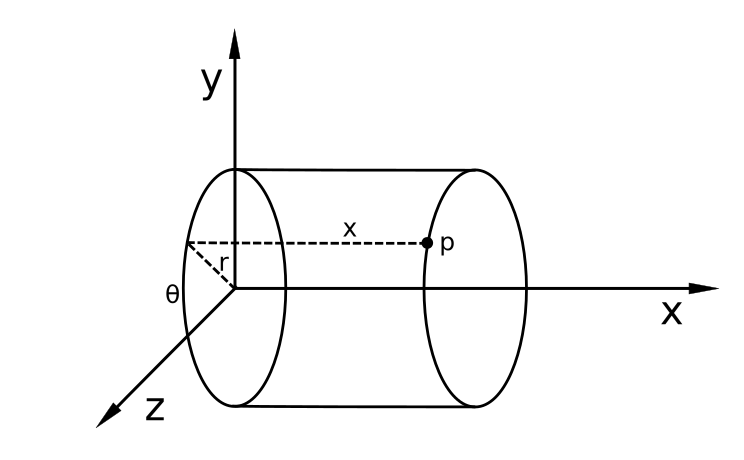
\includegraphics[width=0.5\textwidth]{pictures/cylinder}
	\caption{Darstellung eines zylindrischen Koordinatensystems. $x,y$ und $z$ entsprechen dabei den kartesischen Achsen. Die Koordinaten des Punktes $p$ sind angegeben als $x, r, \theta$. $x$ entspricht der kartesischen Koordinate, $r$ ist die Entfernung zwischen der Projektion von $p$ auf die von $y$ und $z$ Achse aufgespannte Fl\"ache und dem Koordinatenursprung und $\theta$ entspricht dem Winkel zwischen Projektion von $p$, dem Koordinatenursprung und der X-Achse. }
	\label{cylinderCoords}
\end{figure}

Da $K_1 \in [-\infty, \infty]$, $K_2 \in [0,\infty]$, $K_3 \in [-1,1]$ bietet sich f\"ur den K-Invariantensatz eine Darstellung in einem zylindrischen Koordinatensystem an, wobei $K_1$ eine Position auf einer zentralen Achse beschreibt, $K_2$ die orthogonale Entfernung zu diesem Punkt und $K_3$ den Winkel zu einer festgelegten, zur zentralen Achse orthogonalen, zweiten Achse. Sowohl ein zylindrisches als auch ein kartesisches Koordinatensystem sind in Abbildung \ref{cylinderCoords} dargestellt. $K_1$ entspricht dabei der zylindrischen $x$-Koordinate, $K_2$ dem Radius $r$ und $K_3$ dem Winkel $\theta$.

Ein Vorteil des K-Invariantensatzes ist die relativ leichte Interpretierbarkeit in der Kontinuumsmechanik. $K_1$ kann als Ma{\ss} der absoluten `Gr\"o{\ss}e' der Matrix , $K_2$ als Ma{\ss} des anisotropen Anteils angesehen werden \cite{kindlmann2007diffusion}. Dagegen kann aus dem Wert von $K_3$ die Verteilung der Eigenwerte und damit die Form der Anisotropie des Tensors geschlussfolgert werden.



\paragraph{Der R-Invariantensatz}
Der orthogonale R-Invariantensatz verwendet die Invarianten $R_1, R_2$ und $R_3$. F\"ur eine Matrix $A$ sind sie definiert als

\begin{itemize}
	\item $R_1(A)=norm(A)$ (Norm von $A$)
	\item $R_2(A)=\sqrt{\frac{3}{2}} \frac{norm(\tilde{A})}{norm(A)}$ (fraktionale Anisotropie)
	\item $R_3(A)=mode(A)$ (Modus von $A$)
\end{itemize}

Dabei f\"allt auf, dass gilt $R_3(A) = K_3(A) = mode(A)$. \"Ahnlich wie der K-Invariantensatz kann auch R in einem zylindrischen Koordinatensystem dargestellt werden.

\begin{figure}
	\centering
	\includegraphics[width=0.5\textwidth]{pictures/-000.png}
	\caption{Dargestellt sind Isofl\"achen der K und R Invarianten von diagonalisierten $3\times 3$ Matrizen (alle Werte ausserhalb der Hauptdiagonale sind 0). Die Koordinatenachsen entsprechen den drei Eigenwerten der Matrizen. Entnommen aus \cite[S.~139]{ennis2006orthogonal}}
	\label{KRInvariants}
\end{figure}

\"Ahnlich wie der K-Invariantensatz existiert auch f\"ur den R-Satz eine Interpretation in der Kontinuumsmechanik. 

Sowohl K als auch R beschreiben die Verteilung, die Gr\"o{\ss}e und das Verh\"altnis der Eigenwerte zueinander. Dies ist in Abb. \ref{KRInvariants} dargestellt. 

\subsection{Mechanische Grundlagen}
\subsubsection{Physikalisches Feld}
Ein physikalisches Feld ist eine physikalische Gr\"o{\ss}e, die an verschiedenen Positionen im Raum unterschiedliche Werte annimmt\cite[1–2 Electric and magnetic fields]{feynman2011feynman}. Abstrahiert kann es als Funktion $\mathbb{R}^n \rightarrow V$ beschrieben werden, wobei $V$ eine beliebige Menge ist. H\"aufig wird f\"ur $V$ jedoch $\mathbb{R}$ (z.B. bei Temperaturen), $\mathbb{R}^n$ (z.B. bei Str\"omungen) oder $\mathbb{R}^{m\times n}$ (z.B. bei Verformungen) eingesetzt. Andere Beispiele f\"ur physikalische Felder sind elektromagnetische Felder oder Gravitationsfelder. Felder werden meist abh\"angig von ihrem Bild klassifiziert, so z.B. in Skalar-, Vektor- oder Tensorfelder.

Wenn Felder nicht in Form einer kontinuierlichen Funktion beschrieben werden k\"onnen, z.B. weil nur f\"ur endlich viele Punkte Messwerte vorhanden sind, kann ein Feld auf einem Gitter, das aus diesen Messpunkten besteht, definiert werden. Die Werte innerhalb der Zellen lassen sich dann durch Interpolation der Werte an den Eckpunkten berechnen.


Innerhalb der vorliegenden Arbeit werden Spannung und Verformung an Punkten von Objekten als Felder $\mathbb{R} \rightarrow \mathbb{R}^{m\times n}$ beschrieben.


\subsubsection{Mechanische Spannung}
In der Mechanik beschreibt Spannung (engl. stress) die Kraft, die Partikel innerhalb eines Objektes aufeinander auswirken. Um die Spannung an einem Punkt zu bestimmen, wird die Kraft, die auf infinitesimal kleine Fl\"achenteile von Schnitten durch das Objekt wirkt, berechnet. Die Kraft ist dabei als Vektor formulierbar. Wenn die Schnitte entlang von drei zueinander orthogonalen Ebenen durchgef\"uhrt werden, erh\"alt man so drei Vektoren, die zusammen die Matrixdarstellung des Cauchy Tensors $\sigma$ bilden:

\begin{equation}
	\sigma =  
	\begin{bmatrix}
		\sigma_x & \tau_{xy} & \tau_{xz}\\
		\tau_{xy} & \sigma_y & \tau_{yz}\\
		\tau_{xz} & \tau_{yz} & \sigma_z
	\end{bmatrix}
\end{equation}

Jede Spalte des Cauchy Tensors entspricht dabei einem der Vektoren. Wie aus der Formel ersichtlich, ist die Matrix symmetrisch und enth\"alt zwei Typen von Komponenten: Die $\sigma$ entlang der Hauptdiagonale, die Kraft in Richtung der Normalen der jeweiligen Ebene angeben, und den $\tau$, die Scherspannungen angeben, die parallel zu den Schnittebenen verlaufen. 

\subsubsection{Mechanische Verformung}
Wenn in einem Objekt Spannung vorliegt, so verformt es sich proportional zur St\"arke der Spannung (Hookesches Gesetz). Durch einen Verformungstensor (auch Verzerrungstensor, engl. strain tensor) l\"asst sich die Verformung an einem Punkt durch Kraftanwendung angeben:

\begin{equation}
	\   =  
	\begin{bmatrix}
		\epsilon_x & \frac{1}{2}\gamma_{xy} & \frac{1}{2}\gamma_{xz}\\
		\frac{1}{2}\gamma_{xy} & \epsilon_y & \frac{1}{2}\gamma_{yz}\\
		\frac{1}{2}\gamma_{xz} & \frac{1}{2}\gamma_{yz} & \epsilon_z
	\end{bmatrix}
\end{equation}

\"Ahnlich wie beim Spannungstensor dr\"ucken die $\epsilon$ in der Hauptdiagonale Dehnungen oder Stauchungen des Objektes entlang der Hauptachsen aus, die $\gamma$ Werte Scherungen, also Verschiebungen der Seitenfl\"achen zueinander. Dabei \"andern sich die Winkel der Kanten des Objektes zueinander.

\section{Verwendete Verfahren und Technologien}
\label{sec:Technologien}
\subsection{FAnToM}
FAnToM\cite{fantomWebsite}\cite{wiebel2009fantom} (`Field Analysis using Topological Methods') ist ein Programm, dessen Entwicklung im Jahre 1999 begann. Obwohl es zu Anfang noch als Hilfsmittel f\"ur die Analyse von Vektorfeldtopologien konzipiert war, entwickelte es sich \"uber die Jahre hinweg zu einer Plattform f\"ur diverse Visualisierungen.

Erweiterungen von FAnToM werden in Form von sogenannten Algorithmen entwickelt. Dabei unterscheidet man zwei Arten: den `Data Algorithm' und den `Visualization Algorithm'. Data Algorithms sind Erweiterungen, die Daten verarbeiten. Beispiele daf\"ur sind `Load VTK', eine Erweiterung die Daten aus dem VTK Format einliest, oder `Combine Scalar to Vector', das mehrere Felder mit skalaren Werten zu einem einzigen Feld mit Vektorwerten kombiniert, wobei die Vektorkomponenten den Skalaren entsprechen.
Visualization Algorithms dagegen dienen dazu, Visualisierungen zu erzeugen. Interaktionen mit den Visualisierungen k\"onnen entweder \"uber die Maus oder \"uber Optionen stattfinden.

Ein wesentliches Feature von FAnToM besteht darin, Algorithmen miteinander zu verkn\"upfen. Dies geschieht, indem Ausgabedaten von Algorithmen als Eingabe f\"ur andere dienen k\"onnen. Da viele Algorithmen mit Blick auf Wiederverwendbarkeit entwickelt wurden, k\"onnen mit wenig Aufwand aus bestehenden Algorithmen komplett neue Visualisierungspipelines entwickelt werden. Dies geschieht mittels des sogenannten `Flow Graphs', in dem Algorithmen als Knoten dargestellt sind, deren Aus- und Eingaben durch Kanten verbunden werden k\"onnen.

Die aktuelle FAnToM-Session, also die momentan genutzten Algorithmen mit ihren Optionen sowie jeweiligen Ein- und Ausgaben, k\"onnen als `Session' gespeichert und zu einem sp\"ateren Zeitpunkt wieder geladen werden.

Erweiterungen k\"onnen auf eine Vielzahl von m\"achtigen Werkzeugen zugreifen, die von FAnToM zur Verf\"ugung gestellt werden. Besonders wichtig f\"ur die vorliegende Arbeit waren dabei das hoch entwickelte (: anderes Wort) Datenmodell, das viele Funktionen zum Verarbeiten von Feldern und Tensoren bietet, die bestehenden Schnittstellen f\"ur Qt und OpenGL sowie die gro{\ss}e Bibliothek von wiederverwendbaren Algorithmen.
\subsection{OpenGL}
\label{sec:OpenGL}
OpenGL\cite{openglWebsite} ist eine Spezifikation, die das Verhalten eines rasterbasierten Renderingsystems beschreibt. Sie definiert eine Schnittstelle, gegen die von zwei Seiten entwickelt werden kann: Zum einen von Seiten der Hardwarehersteller, die Funktionen von OpenGL auf ihrer Hardware implementieren. Zum anderen von Programmierern, die durch OpenGL unabh\"angig von der Hardware, auf der das Programm laufen soll, entwickeln k\"onnen. 

Die Verarbeitungsschritte von der \"Ubergabe von Daten zu OpenGL bis zum fertig gerenderten Bild wird als Renderpipeline bezeichnet. Seit Version 2.0 unterst\"utzt OpenGL sogenannte `Shader', kleine Programmst\"ucke, die es Nutzern von OpenGL erm\"oglichen, die Renderpipeline sehr stark zu ver\"andern. Shader bekommen drei Arten von Eingabedaten:

\begin{enumerate}
	\item Die Ausgabe des vorherigen Schrittes in der Renderpipeline
	\item Parameter aus dem Programm, das OpenGL verwendet (`Uniforms')
	\item Daten, die aus dem vorhergehenden Shader \"ubergeben wurden
\end{enumerate}

Ein wichtiger Spezialfall von Uniforms sind Texturen, die in dem OpenGL verwendenden Programm geladen, an die Shader \"ubergeben und dort verwendet werden k\"onnen.

In der vorliegenden Arbeit wurden Vertex, Geometry und Fragment Shader entwickelt. Diese drei Typen sind im Folgenden kurz erkl\"art.

\paragraph{Vertex Shader}
Vertex Shader bekommen als Eingabe aus der Renderpipeline die Punkte eines zu zeichnenden Grafikprimitivs, beispielsweise Punkte eines Liniensegmentes oder die Eckpunkte eines Dreiecks. Abh\"angig von den eingegebenen Uniforms k\"onnen die Koordinaten dieser Punkte dann durch den Shader ver\"andert werden. Dies ist zum Beispiel \"ublich um die Sicht auf die Szene von der Position der Kamera aus zu berechnen. Vertex Shader werden einmal pro Punkt ausgef\"uhrt. Die Ausgabe des Vertex Shaders sind die neuen Koordinaten der Punkte der Primitive.

\paragraph{Geometry Shader}
Die Renderpipeline \"ubergibt dem Geometry Shader f\"ur jedes Primitiv eine Liste der zugeh\"origen Punkte, z.B. eine Liste von drei Punkten f\"ur ein Dreieck. Der Geometry Shader ist in der Lage, die Position und den Typ dieser Primitive beliebig zu ver\"andern und sogar neue Punkte zu erzeugen. So kann er bespielsweise aus einer Linie ein Dreieck erzeugen sowie Uniforms pro Punkt definieren, welche an sp\"ater ausgef\"uhrte Shader (Fragment Shader) weitergegeben werden. Pro Primitiv wird der Geometry Shader einmal ausgef\"uhrt.

\paragraph{Fragment Shader}
Fragment Shader bestimmen die Farben der Fragmente. Fragmente sind St\"ucke der projizierten Primitve, deren Gr\"o{\ss}e von der Art der Rasterisierung abh\"angen (z.B. Supersampling). Die Eingaben sind der Mittelpunkt des Fragments und die f\"ur diesen Punkt interpolierten Attribute der Eckpunkte des Primitivs. Neben der Fragmentfarbe k\"onnen auch Werte ausgegeben werden, z.B. ein Tiefenattribut, das korrekte \"Uberlappung von Primitiven erm\"oglicht.

Eine weitere im Folgenden verwendete Funktion von OpenGL ist `Blending', durch die Fragmente \"ubereinander gezeichnet und ihre Farbwerte gewichtet kombininert werden k\"onnen, was z.B. f\"ur transparente Objekte wichtig ist. Zudem existiert die M\"oglichkeit, gerenderte Bilder mithilfe von `Framebuffern' nicht anzuzeigen, sondern stattdessen in einer Textur zu speichern.

Die meisten Implementierungen von OpenGL machen intensiven Gebrauch von Grafikkarten und deren F\"ahigkeit zur extremen Parallelisierung von Aufgaben. Dies, verbunden mit der M\"oglichkeit Ausgaben der Renderpipeline zur\"uck in den Arbeitsspeicher zu laden und der Anpassbarkeit der Renderpipeline durch Shader, erm\"oglicht es, OpenGL auch f\"ur andere rechenintensive, jedoch gut parallelisierbare Aufgaben zu benutzen und so Berechnungen stark zu beschleunigen.

\subsection{Qt}
Qt\cite{qtWebsite} ist eine popul\"are, plattform\"ubergreifende Bibliothek f\"ur die Entwicklung von Programmoberfl\"achen. Die Popularit\"at von Qt beruht auf der Plattformunabh\"angigkeit und der gro{\ss}en Vielfalt leicht zu verwendender Funktionen.

FAnToM besitzt eine auf Qt basierende Oberfl\"ache, die aus Algorithmen heraus um weitere Fenster und Elemente erweitert werden kann. Eine wesentliche F\"ahigkeit von Qt ist dabei, einen OpenGL Kontext zu erzeugen, sodass durch OpenGl gerenderte Bilder angezeigt werden k\"onnen. Diese F\"ahigkeit von Qt wird innerhalb dieser Arbeit verwendet, um mehrere, unabh\"angige Datensichten zu implementieren.

\subsection{Direct Volume Rendering}
In der Computergrafik werden dreidimensionale Objekte \"ublicherweise durch Dreiecke dargestellt, durch die die Oberfl\"achen der Objekte approximiert werden. Solches Vorgehen entfernt jedoch alle Informationen \"uber Strukturen im Inneren der Objekte, so wie Bereiche unterschiedlicher Materialien oder Dichte. Durch das Berechnen und Zeichnen von Isofl\"achen kann dieses Problem behoben werden, dies erfordert jedoch hohe Rechenzeiten und gute Kenntnis der Datens\"atze, um geeignete Isowerte festzulegen.


\begin{figure}
	\begin{minipage}{0.5\textwidth}
		\centering
		\includegraphics[width=0.9\textwidth]{pictures/Colormap.png}
		\caption{Eine Implementierung einer interaktiven Transferfunktion in FAnToM. }
		\label{Colormap}
	\end{minipage}
	\hspace{0.5cm}
	\begin{minipage}{0.5\textwidth}
		\centering
		\includegraphics[width=0.47\textwidth]{pictures/Zahn.png}
		\caption{Ein Direct Volume Rendering eines Zahns. Entnommen aus \cite[S.~6]{drebin1988volume}}
		\label{Zahn}
	\end{minipage}
\end{figure}
Eine Alternative bietet das Direct Volume Rendering\cite{drebin1988volume} (im Folgenden DVR). Als Eingabe wird ein Feld $f: \mathbb{R}^3\rightarrow\mathbb{R}$ verwendet, das Punkten im dreidimensionalen Raum skalare Werte zuordnet. Die Interpretation dieser Werte kann, abh\"angig vom Einsatzgebiet, unterschiedlich sein. Beispiele daf\"ur sind die abgegebene Energie von Regionen in der Magnetresonanztomographie oder die Menge von absorbierter R\"ontgenstrahlung in der Computertomographie. Den skalaren Werten werden mittels einer `Transferfunktion' Farbwerte und Transparenz zugeordnet.

Eine Implementierung einer interaktiven Transferfunktion in FAnToM ist in Abb. \ref{Colormap} zu sehen. Die horizontale Achse entspricht den skalaren Werten zwischen Minimum und Maximum im Datensatz sowie den zugeordneten Farben. Die vertikale Achse entspricht der Transparenz, von vollst\"andig transparent am unteren Rand bis zu opak am oberen Rand. Durch Position und Farbe der Dreiecke am oberen Rand der Transferfunktion kann die Farbzuordnung festgelegt werden. Die Quadrate stellen interaktiv ausgew\"ahlte Punkte dar, die Zuordnungen von Werten im Skalarfeld zu Farb- und Transparenzwerten entsprechen, zwischen denen entlang der verbindenden Linien interpoliert wird. So wird allen Werten im Feld eine Farbe und eine Transparenz zugeordnet. 

Ziel des DVR ist es, mithilfe der Transferfunktion eine dreidimensionale Darstellung des Feldes zu erzeugen, in der Bereiche entsprechend der Transferfunktion Licht ausstrahlen. Abh\"angig von ihrer Transparenz absorbieren andere Bereiche dieses Licht oder lassen es durch. Dadurch ist es m\"oglich, Strukturen im Inneren des Feldes sichtbar zu machen. Ein Beispiel f\"ur eine so erzeugtes Bild ist in Abb. \ref{Zahn} dargestellt.

Es existieren viele DVR Verfahren die sich in Laufzeit, Bildqualit\"at und Anf\"alligkeit f\"ur Artefakte unterscheiden. In dieser Arbeit wurde Raycasting verwendet, was folgend erl\"autert wird.

\subsubsection{Raycasting}
\label{sec:Raycasting}
\begin{figure}
	\centering
	\includegraphics[width=0.5\textwidth]{pictures/Raycasting}
	\caption{Eine vereinfachte Darstellung eines optimierten Raycastings. Die Bildebene entspricht der Ebene, die durch die imagin\"are Position der Pixel gebildet wird. Die roten Punkte entlang der Strahlen entsprechen den Samplepoints.}
	\label{Raycasting}
\end{figure}
Beim Raycasting wird f\"ur jedes Pixel ein Strahl durch den Mittelpunkt des Pixels und die Position der Kamera berechnet. Entlang dieses Strahls wird, an nach ihrer Entfernung von der Kamera geordneten Punkten  $s_1, \dots, s_n$ (`Samplepoints') der interpolierte Wert des Feldes $v(s_i), 1\leq i\leq n$ berechnet. Der paarweise Abstand der Samplepunkte ist dabei konstant. Aus dem ermittelten Wert wird mithilfe der Transferfunktion die Farbe $f(v(s_i))$ und die Transparenz $t(v(s_i))$ f\"ur diesen Wert bestimmt.

Dabei sei die Transparenz ein Wert im Intervall $[0,1]$ und Farbe ein Vektorraum \"uber $\mathbb{R}$, wie z.B. im RGBA Farbmodell, f\"ur den die Multiplikation mit einem Skalar definiert ist. Die Farbe des Pixels $p$ wird dann f\"ur die Samplepunkte entlang des entsprechenden Strahls berechnet als

\begin{equation}
	p = \sum_{i=1}^{n} \left(f(s_i) \cdot \prod_{j=1}^{i} \frac{(1-t(s_j))}{n}\right)
	\label{RaycastingFormula}
\end{equation}

Das hat den Effekt, dass weiter von der Kamera entfernte Samplepunkte von n\"aheren Punkten entsprechend ihrer Transparenz verdeckt werden. Insbesondere folgt daraus die Konsequenz, dass, sobald gen\"ugend Punkte verarbeitet wurden, so dass die `verbleibende Transparenz' einen Grenzwert unterschreitet, sich die Farbe des Pixels nicht mehr stark ver\"andert, und die Berechnung fr\"uhzeitig beendet werden kann. Die verbleibende Transparenz wird durch die Gesamtzahl der Samplepunkte $n$ geteilt, damit eine h\"ohere Anzahl an Samplepoints nicht zu einem schnelleren Verlust von Transparenz f\"uhrt.

Eine weitere Optimierung besteht darin, den ersten Samplepunkt erst nach dem Eintreten des Strahls in das Feld zu setzen und die Berechnung zu beenden, sobald alle verbleibenden Samplepunkte ausserhalb des Feldes liegen. Eine vereinfachte Darstellung dieses optimierten Verfahrens ist in \ref{Raycasting} dargestellt.
 
\begin{figure}
	\begin{subfigure}{0.30\textwidth}
		\includegraphics[width=\textwidth]{pictures/DVR1.png}
		\subcaption{}
		\label{SamplingPoints1}
	\end{subfigure}
	\hfill
	\begin{subfigure}{0.30\textwidth}
		\includegraphics[width=\textwidth]{pictures/DVR2.png}
		\subcaption{}
		\label{SamplingPoints2}
	\end{subfigure}
	\hfill
	\begin{subfigure}{0.30\textwidth}
		\includegraphics[width=\textwidth]{pictures/DVR3.png}
		\subcaption{}
		\label{SamplingPoints3}
	\end{subfigure}
	\caption{Drei Raycastings des Felds $f:\mathbb{R}^3\rightarrow\mathbb{R}, f\left(\protect\begin{array}{c}x\\y\\z\protect\end{array}\right)=cos(x\cdot y\cdot z)$.}
	\label{SamplingPoints}
\end{figure}

Die Qualit\"at eines Raycastings ist stark abh\"angig von der Anzahl an Samplepoints pro Strahl und somit vom Abstand zwischen den Samplepoints. Ein geringerer Abstand f\"uhrt generell zu weniger Artefakten und macht kleine Strukturen besser erkennbar, erh\"oht jedoch den Rechenaufwand. Indem der Nutzer die Anzahl von Samplepoints selbst ausw\"ahlt, kann er seinen optimalen Tradeoff zwischen Rechenzeit und Bildqualit\"at finden. In Abb. \ref{SamplingPoints1} und \ref{SamplingPoints2} sind zwei Darstellungen desselben Skalarfeldes zu sehen, die durch Raytracing mit einer unterschiedlichen Anzahl von Samplepoints erzeugt wurden. \ref{SamplingPoints1} wurde mit 20 Samplepoints erstellt, wodurch visuelle, scheibenartige Artefakte entstanden. Bei einer h\"oheren Menge von 200 Samplepoints in \ref{SamplingPoints2} verschwinden diese Artefakte.

Eine weitere wichtige Einstellung ist, welche Zahl in Formel \ref{RaycastingFormula} f\"ur Variable $n$ verwendet wird. Wenn $n$ die Anzahl der Samplepunkte pro Strahl ist, kann dies, wenn die Blickrichtung der Kamera nicht senkrecht auf einer der Seitenfl\"achen steht, dazu f\"uhren, dass Bereiche am Rand des Feldes transparenter dargestellt werden als in der Mitte. Das liegt daran, dass der Strahl am Rand weniger Samplepunkte produziert, die innerhalb des Feldes liegen. Ein Beispiel daf\"ur ist in \ref{SamplingPoints3} mit 200 Samplepoints dargestellt. 

Alternativ kann f\"ur $n$ die Anzahl der Samplepunkte, die tats\"achlich im Feld liegen, gew\"ahlt werden. Dies wurde in Abb. \ref{SamplingPoints2} getan. Wenn man nun \ref{SamplingPoints2} und \ref{SamplingPoints3} miteinander vergleicht, f\"allt auf, dass die Pixel in der Mitte der Darstellung etwa die gleichen Farben erhalten haben, \ref{SamplingPoints3} in Richtung Rand jedoch erheblich transparenter wird. Welche von beiden Varianten bevorzugt wird, h\"angt von der Art des Datensatzes ab sowie davon, wie wichtig es ist, korrekte Werte ablesen und vergleichen zu k\"onnen.

\subsection{Continuous Scatterplotting}
\subsubsection{Scatterplotting}
\begin{figure}
	\hspace{2cm}
	\begin{subfigure}{0.30\textwidth}
		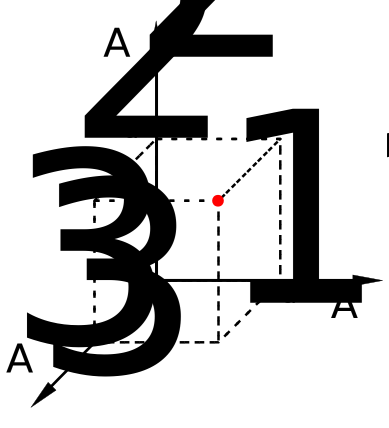
\includegraphics[width=\textwidth]{pictures/Scatterplot3D}
		\caption{}
	\end{subfigure}
	\hfill
	\begin{subfigure}{0.30\textwidth}
		\includegraphics[width=\textwidth]{pictures/Scatterplot2D}
		\caption{}
	\end{subfigure}
	\hspace{2cm}
	\caption{Zwei Beispiele f\"ur Scatterplottings. In (a) wird ein Objekt mit den Attributwerten $a_1, a_2, a_3$ als roter Punkt in einem dreidimensionalen Scatterplot dargestellt. Um die Attribute besser ablesen zu k\"onnen, wurden gestrichelte Linien eingezeichnet. In (b) wurden mehrere Objekte mit unterschiedlichen Attributen im selben, zweidimensionalen Scatterplot als schwarze Punkte eingezeichnet.}
	\label{Scatterplots}
\end{figure}

Scatterplotting ist ein weit verbreitetes Verfahren, um Attribute von Objekten relativ zueinander darzustellen. Es ist eine Funktion auf einer Menge von Objekten $M$ als $\tau: M \rightarrow \mathbb{R}^n,n\in\{1,2,3\}$, wobei das Bild eine Projektion auf einzelne oder zusammengesetzte Attribute der Objekte darstellt.  Dazu wird je Objekt ein Punkt in ein ein-, zwei- oder dreidimensionales Koordinatensystem eingetragen, dessen Koordinatenachsen Attributwerten entsprechen. Beispiele f\"ur Scatterplottings sind in Abb. \ref{Scatterplots} abgebildet. Das Bild von $\tau$ ist auf maximal drei Dimensionen beschr\"ankt, da h\"oherdimensionale Daten visuell nur schwer zu interpretieren sind.

Ein Vorteil von Scatterplottings ist die leichte Erkennbarkeit von Strukturen in den Datens\"atzen: Cluster, Outlier und funktionale Zusammenh\"ange zwischen den verwendeten Attributen lassen sich gut identifizieren. 

Scatterplotting hat jedoch zwei gravierende Nachteile. Zum einen macht die geringe Dimensionalit\"at des Bildes von $\tau$ die Projektion auf eine Teilmenge der Attribute notwendig, zum anderen kann Scatterplotting nur endlich viele Objekte gleichzeitig darstellen. 

Ein Beispiel f\"ur ein Urbild mit unendlich vielen Elementen ist $\mathbb{R}^n$ bei physikalischen Feldern. Dort sind an jedem der unendlich vielen Punkte Werte definiert. Ein Scatterplot dieser unendlich vielen Elemente ist nun weder in endlicher Laufzeit m\"oglich, noch w\"aren einzelne Punkte in der entstehenden Darstellung erkennbar. Eine Alternative besteht darin, nur den Scatterplot der Eckpunkte der Zellen zu erzeugen, doch damit gehen Informationen \"uber die Punkte innerhalb der Zellen verloren.


\subsubsection{Erkl\"arung des Continuous Scatterplottings}
\begin{figure}
	\centering
	\begin{subfigure}{0.45\textwidth}
		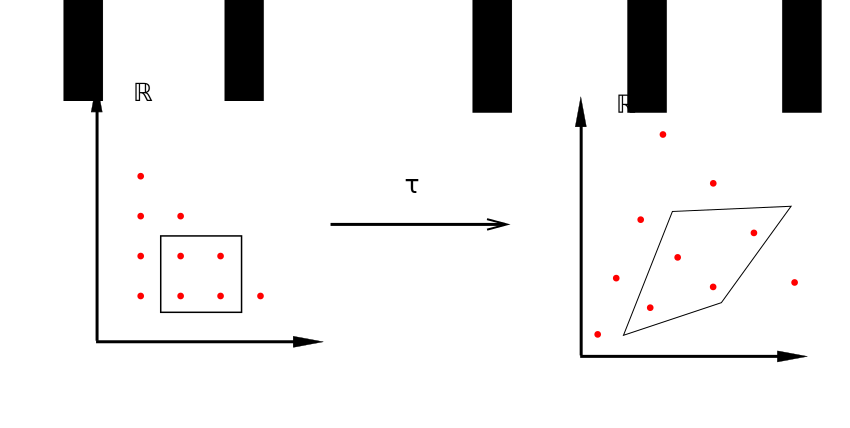
\includegraphics[width=0.9\textwidth]{pictures/ContinuousScatterplot}
		\subcaption{}
	\end{subfigure}
	\begin{subfigure}{0.45\textwidth}
		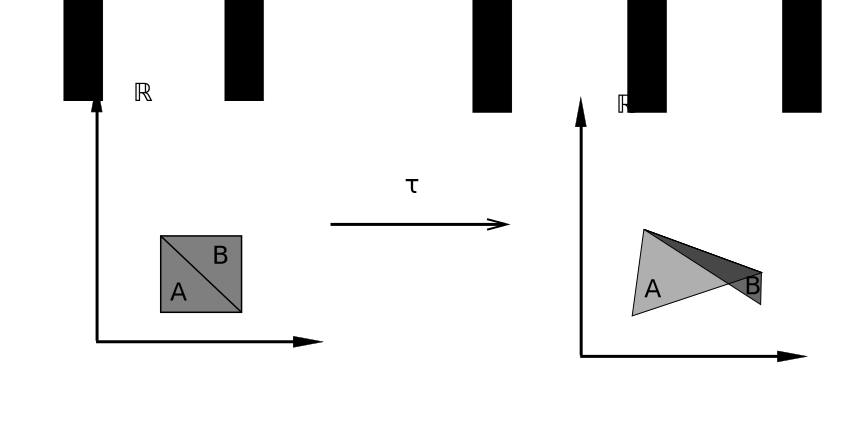
\includegraphics[width=0.9\textwidth]{pictures/Case2}
		\subcaption{}
		\label{Case2}
	\end{subfigure}
	\caption{Darstellung der Dichteverteilung abh\"angig von $\tau$. (a) Die roten Punkte deuten die Dichte in den beiden Scatterplots an, die zwei Vierecke sind ein Bereich des Urbilds, der durch $\tau$ verformt wird. Zu erkennen ist, dass eine Streckung eines Bereichs zur Verringerung der Dichte und eine Stauchung zur Erh\"ohung der Dichte f\"uhrt. (b) Der Continuous Scatterplot zweier Dreiecke. Der Grauwert gibt die Dichte in den jeweiligen Bereichen an. }
	\label{ContinuousScatterplot}
\end{figure}
Das Continuous Scatterplotting stellt eine Erweiterung des Scatterplottings dar, sodass statt nur einer endlichen Anzahl von Objekten auch kontinuierliche Bereiche verarbeitet werden k\"onnen. Die von Bachthaler und Weiskopf\cite{bachthaler2008continuous} vorgestellte Definition wurde von Fritzsch\cite{fritzsch2016continuousScatterplot} um einige wichtige Punkte erweitert. Beim Continuous Scatterplotting wird ein Ansatz verwendet, der dem Verfahren bei der Herleitung der Kontinuumsmechanik aus Systemem mit diskreten Massepunkten \"ahnelt \cite[S.~1429]{bachthaler2008continuous}. Das Ziel des Continuous Scatterplottings ist es, eine Dichtefunktion $\sigma: \mathbb{R}^m \rightarrow \mathbb{R}$ zu finden, die den Punkten des Bildraums, abh\"angig von $\tau$, Dichtewerte zuordnet. $\sigma$ kann als Funktion aufgefasst werden, die jedem Pixel des Scatterplots einen skalaren Wert zuordnet, der z.B. als Farbe oder Opazit\"at dargestellt werden kann. In Abb. \ref{ContinuousScatterplot} ist der Effekt, den $\tau$ auf die Dichtefunktion hat, dargestellt. Um $\sigma$ berechnen zu k\"onnen, werden zwei Annahmen getroffen:

Die erste Annahme ist, dass eine Dichtefunktion $s: \mathbb{R}^n \rightarrow \mathbb{R}$ existiert, die jedem Punkt des Urbilds von $\tau$ einen skalaren Wert, die Dichte an diesem Punkt, zuordnet. Der Einfachheit halber wird wird im Folgenden eine uniforme Dichte von $s(x) = 1$ angenommen. Aus der Dichte an den Punkten l\"asst sich die Gesamtdichte $M$, auch bezeichnet als Masse, einer Teilmenge $V\subset\mathbb{R}^n$ berechnen:

\begin{equation}
	M = \int_{V}s(x)d^nx
	\label{Dichtefunktion}
\end{equation}

Die zweite Annahme besagt, dass die Masse einer Teilmenge $V\subset\mathbb{R}^m$ gleich der Masse ihres Urbildes ist, also $\tau$ die Gesamtdichte nicht beeinflusst. Da $\tau$ in der Regel nicht invertierbar ist, wird $\tau^{-1}(\phi), \phi \subset \mathbb{R}^m$ verwendet, um das Urbild von $\phi$ zu notieren. 


F\"ur $\xi \in \Phi$ f\"uhren die Annahmen zu der Gleichung

\begin{equation}
	\int_{\phi}\sigma(\xi)d^m\xi = \int_{\tau^{-1}(\phi) = V}s(x)d^nx
\end{equation}

Da $\tau$ weder injektiv noch surjektiv ist, gilt der umgekehrte Fall nur, wenn zus\"atzlich $\forall x \in V: f^{-1}(f(x)) \subset V$ gilt\cite [S.~20]{fritzsch2016continuousScatterplot}.

\begin{equation}
	\int_{V}s(x)d^nx = \int_{\phi = \tau(V)}\sigma(\xi)d^m\xi
\end{equation}

Fritzsch \cite[S.~20~f.]{fritzsch2016continuousScatterplot} definiert zus\"atzlich ein $\sigma_v$, das die Dichtefunktion der Einschr\"ankung von $\tau$ auf $V$ beschreibt, also den `Beitrag' von $V$ zu $\sigma$.

\begin{equation}
	\int_{\phi} \sigma_v(\xi)d^m\xi = \int_{\tau|_V^{-1}(\phi)}s(x)d^nx
\end{equation}

Mithilfe der $\sigma_v$ stellt Fritzsch fest, dass f\"ur eine Zerlegung des Definitionsbereichs $U$ von $\tau$ in eine Menge von disjunkten Teilmengen $\hat{V} = {V_i | V_i \in U}$ gilt, dass

\begin{equation}
\begin{split}
\int_{\phi}\sigma(\xi)d^m\xi 
&= \int_{\bigcup\limits_{V_i}\tau|_{V_i}^{-1}(\phi)} s(x)d^nx
\\
&= \sum_{V_i}\int_{\tau|_{V_i}^{-1}(\phi)} s(x)d^nx
\\
&= \sum_{V_i}\int_{\phi}\sigma_{V_i}(\xi)d^m\xi
\\
&= \int_{\phi}\sum_{V_i}\sigma_{V_i}(\xi)d^m\xi
\end{split}
\end{equation}

Da die Integranden des ersten und letzten Integrals gleich sein m\"ussen, ergibt sich daraus

\begin{equation}
	\sigma(\xi) = \sum_{V_i}\sigma_{V_i}(\xi)
	\label{DensitySum}
\end{equation}

Eine intuitive Interpretation von Formel \ref{DensitySum} ist, dass die gesamte Dichtefunktion von $\tau$ als Summe der Dichtefunktionen der Einschr\"ankungen von $\tau$ auf die $V_i$ gebildet werden kann.

Die Berechnung von $\sigma$ h\"angt vom Verh\"altnis von $m$ und $n$ zueinander ab. Da in der vorliegenden Arbeit nur der Fall $m=n=3$ auftritt, beschr\"ankt sich die weitere Er\"auterung auf diesen Fall. F\"ur $m=n$ unterscheiden Bachthaler und Weiskopf folgende F\"alle f\"ur $V \subseteq \mathbb{R}^n$\cite[S.~1430]{bachthaler2008continuous}:

\paragraph{Fall 1: $\tau$ ist differenzierbar und ein Diffeomorphismus}
Ein Diffeomorphismus ist eine bijektive, stetig differenzierbare Abbildung, deren Umkehrabbildung ebenfalls stetig differenzierbar ist. 
Wenn $\tau$ ein Diffeomorphismus ist, l\"asst sich durch die Anwendung des Transformationssatzes von Integralen die Gleichung 

\begin{equation}
	\int_{\tau(V)}\sigma(\xi)d^{m=n}\xi = \int_{V}\sigma(\tau(x))|det(J_\tau)(x)|d^nx = \int_{V}s(x)d^nx
\end{equation}

bilden, wobei $J_\tau$ die Jacobimatrix von $\tau$ ist. Da der Wert der Determinante der Jacobimatrix von der Position abh\"angig ist, wird der jeweilige Punkt $x$ eingesetzt. Durch weitere Umformungen entsteht die Gleichung

\begin{equation}
	\sigma(\xi) = \frac{s(\tau^{-1}(\xi))}{|\det(J_\tau)(\tau^-1(\xi))|}
	\label{Case1Formula}
\end{equation}

Wie schon in \hyperref[sec:Grundlagen]{3 Grundlagen} erw\"ahnt, entspricht der Betrag der Determinanten der Jacobimatrix dem Betrag Expandierung oder Schrumpfung der Funktion in der N\"ahe des jeweiligen Punktes. Wenn die Funktion expandiert nimmt die Dichte ab, wenn sie schrumpft nimmt die Dichte zu.

\paragraph{Fall 2: $\tau$ ist differenzierbar und konstant \"uber V, V ist keine Nullmenge}
Wenn $det(J_\tau) = 0$, dann ist $\tau$ kein Diffeomorphismus und $\sigma$ kann nicht so wie in Fall 1 definiert werden. Das ist z.B. der Fall, wenn $\tau$ Bereiche mit konstanten Werten enth\"alt und f\"uhrt dazu, dass ein Bereich aus $\mathbb{R}^n$ auf einen einzelnen Punkt $\xi$ abgebildet wird. Eine M\"oglichkeit die unendlich hohe Dichte an $\xi$ darzustellen und dennoch die Gesamtmasse nicht zu ver\"andern ist es, bei $\xi$ ein Dirac-Delta einzuf\"ugen, das mit dem Volumen aller konstanten Bereiche $V_i \in V$, die nach $\xi$ abgebildet werden, skaliert wird:

\begin{equation}
	\begin{split}
	\sigma(\xi) &= \sum_{V_i \in V}\delta(\xi - \tau(V_i)) \cdot \int_{V_i}s(x)d^nx\\
				&= \sum_{V_i \in V}\delta(\xi - \tau(V_i)) \cdot Vol(V_i)~~~~~~~~~(da~s(x) = 1)
	\end{split}
	\label{DiracTimesVolume}
\end{equation}

Aus den Eigenschaften des Dirac Deltas ergibt sich, dass die Masseerhaltung erf\"ullt ist:

\begin{equation}
	\begin{split}
	\int_{\phi}\sigma(\xi)d^n\xi &= \sum_{V_i}\int_{\phi}\delta(\xi - \tau(V_i)) \cdot Vol(V_i)d^n\xi\\
								 &= \sum_{\forall V_i~:~\tau(V_i)\in \phi} Vol(V_i)\\
								 &= \int_{\tau^-1(\phi)}1~d^nx
	\end{split}
\end{equation}

Da $s(x) = 1$ festgelegt ist, ist die Bedingung erf\"ullt. In \ref{Case2} ist ein Beispielfall daf\"ur angegeben. Die Dichte im \"uberlappenden Bereich der beiden Dreiecke ist gleich der Summe der Dichten der einzelnen Dreiecke. Bei anderen Dichtefunktionen muss Formel \ref{DiracTimesVolume} entsprechend angepasst werden.

\paragraph{Fall 3: $\tau$ ist differenzierbar und kein Diffeomorphismus, V ist Nullmenge}
Ein weiterer Fall, in dem $det(J_\tau) = 0$ ist, tritt auf wenn $V$ eine Nullmenge ist (also z.B. eine Linie im $\mathbb{R}^3$). Da Integration \"uber Nullmengen immer 0 ergibt, k\"onnen die Nullmengen und ihr Bild bez\"uglich $\tau$ einfach aus dem Scatterplotting entfernt werden, ohne die Masseerhaltung zu verletzen.

\paragraph{Fall 4: $\tau$ ist nicht differenzierbar}
Wenn im Datensatz Unstetigkeiten auftreten, zum Beispiel zwischen Zellen, ist $\tau$ an diesen nicht differenzierbar. Da die unstetigen Bereiche ebenfalls Nullmengen bilden, kann die gleiche L\"osung wie in Fall 3 gew\"ahlt werden.

\begin{figure}
	\begin{subfigure}{0.66\textwidth}
		\includegraphics[width=\textwidth]{pictures/Case5}
		\subcaption{}
		\label{Case5}
	\end{subfigure}
	\begin{subfigure}{0.33\textwidth}
		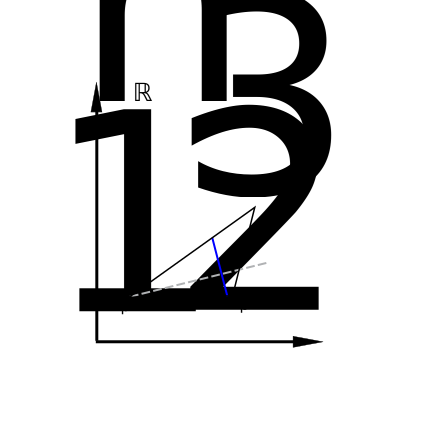
\includegraphics[width=\textwidth]{pictures/Case5-Solution}
		\subcaption{}
		\label{Case5Solution}
	\end{subfigure}
	\caption{Eine Darstellung des f\"unften Falls. (a) Alle drei Punkte des Dreiecks $V$ im linken Koordinatensystem werden auf eine Gerade abgebildet. Dadurch ist $\tau(V)$ eine Nullmenge. (b) Eine Darstellung des von Fritzsch vorgeschlagenen Ansatzes. Die graue, gestrichelte Linie entspricht dem Gradienten, die L\"ange der blauen Linie ist proportional zur Dichte. }
\end{figure}

\paragraph{Fall 5: $\tau$ ist differenzierbar und kein Diffeomorphismus, V ist keine Nullmenge}\mbox{}\\
Von Bachthaler und Weiskopf wurde noch ein f\"unfter Fall genannt, den sie jedoch als nicht in der Praxis vorkommend ansahen. Fritzsch konnte jedoch Beispiele f\"ur diesen Fall angeben\cite[S.~23~f.]{fritzsch2016continuousScatterplot}, die in der Praxis eine Rolle spielen. Ein solcher Fall tritt ein, wenn $V$ keine Nullmenge ist, jedoch auf eine Nullmenge $\tau(V)$ abgebildet wird (siehe Abb. \ref{Case5}), wenn also entweder mindestens eine Komponente des Bildes konstant ist, oder eine funktionale Abh\"angigkeit zwischen mindestens zwei Komponenten existiert. 

Die Jacobimatrix enth\"alt in diesem Fall mindestens eine Nullzeile, wodurch f\"ur ihren Rang gilt $0 < rang(M) < m$. 

Fritzsch schl\"agt zur L\"osung dieses Problems zwei Ans\"atze vor. 

Der erste orientiert sich an Fall 2 und ordnet dem Bildbereich sehr hohe Dichten zu, um die Masseerhaltung zu gew\"ahrleisten. 

Der zweite Ansatz ist nur f\"ur den Fall $m=2, n=2$ beschrieben (somit muss $rang(M) = 1$ sein). Er kann jedoch auch auf h\"ohere Dimensionen \"ubertragen werden. Ziel ist es, die Dichte an Punkten $p\in\tau(V)$ proportional zur Gesamtmasse der darauf abgebildeten Punkte festzulegen. Dadurch wird zwar die Masseerhaltung nicht erf\"ullt, aber eine interpretierbare Darstellung erzeugt. Dazu werden zun\"acht die Gradienten f\"ur jede Komponente des Bildes von $V$ berechnet. Die Gr\"o{\ss}e der $dim(V) - dim(\tau(V))$-dimensionalen Teilmengen von $V$, die orthogonal zu den durch die Gradienten aufgespannten R\"aumen sind, ist gleich der Masse, die auf die einzelnen Punkte abgebildet wird. Ein Beispiel f\"ur den Fall $dim(V) = 2,~dim(\tau(V)) = 1$ ist in \ref{Case5Solution} zu sehen. Die Dichte an den Punkten von $\tau(V)$ wird dann proportional zur Masse gew\"ahlt.

\section{Umsetzung}
\label{sec:Umsetzung}
In diesem Kapitel wird beschrieben, wie die Grundlagen, Technologien und Verfahren aus den vorherigen Kapiteln eingesetzt wurden, um eine interaktive Tensorfeldvisualisierung in FAnToM zu erzeugen.

Die Grundidee der entwickelten Visualisierung besteht darin, zwei DVRs zu erzeugen. Das erste stellt die Zellen des ursp\"unglichen Feldes dar, \"uber die eine konstante Dichte angenommen wird. Da das Zielgebiet der Anwendung die Materialforschung ist, wird das urspr\"ungliche Feld im Folgenden als `Objekt' bezeichnet. F\"ur das zweite DVR werden die 3 Invarianten eines Invariantensatzes der an den Eckpunkten der Zellen definierten Tensoren berechnet und diese als Koordinaten interpretiert. Die Zellstruktur wird somit in einen `Invariantenraum' \"uberf\"uhrt. Wegen der Popularit\"at der K- und R-Invariantens\"atze werden die Koordinaten zus\"atzlich in ein zylindrisches Koordinatensystem \"uberf\"uhrt. Dieses Feld wird deshalb im Folgenden als `Feld im Invariantenraum' bezeichnet. Die Dichten in den Zellen der neuen Zellstruktur werden durch Methoden des Continuous Scatterplottings berechnet.

In die Darstellung des zylindrischen Invarianten DVRs werden ausserdem noch Interaktionsfl\"achen in Form von Kreissektoren eingezeichnet. Durch Interaktion mit der Maus k\"onnen die Fl\"achen verschoben sowie ihr Radius und die Winkel der beiden Kreisradienten zur XY Ebene ver\"andert werden.
Mithilfe der Interaktionsfl\"achen kann der Nutzer Bereiche von Invarianten ausw\"ahlen. Alles, was ausserhalb des ausgew\"ahlten Bereichs liegt, wird im zylindrischen DVR ausgeblendet. Auch in der Darstellung des Objekts werden alle Bereiche ausgeblendet, deren Invarianten ausserhalb des gew\"ahlten Bereichs liegen. 

Zus\"atzlich existieren weitere Optionen, durch die der Nutzer die Darstellungen an seine Problemstellung anpassen kann.

Das Verfahren zur Erzeugung der Darstellungen und Interaktionen ist im Folgenden n\"aher erl\"autert.

\subsection{Datenvorbereitung}
\begin{figure}
	\centering
	\includegraphics[width=\textwidth]{pictures/BigSession.png}
	\caption{Der Flowgraph der FAnToM Session, die zur Vorbereitung der Daten verwendet wird.}
	\label{BigSession}
\end{figure}
\subsubsection{Die Vorbereitungssession}
Bevor die Visualisierung beginnen kann, m\"ussen die Daten vorbereitet werden. Um Zeit zu sparen, wird dieser Schritt f\"ur jeden Datensatz nur einmal durchgef\"uhrt und die Ergebnisse abgespeichert. Die Vorbereitung geschieht durch eine Reihe von FAnToM Algorithmen, die im Folgenden beschrieben werden. Ein Screenshot der f\"ur die Datenvorbereitung verwendeten Session ist in Abb. \ref{BigSession} zu sehen. Die Algorithmen der Session werden im weiteren Verlauf erkl\"art.

Die verwendeten Eingabedaten liegen im VTK Format\cite{avila2010vtk} vor. Daher l\"adt der erste Algorithmus `Load/VTK' die VTK Dateien. Der Algorithmus `Extract Domain' extrahiert die Zellstruktur, auf der das Tensorfeld definiert ist. Falls die Zellen keine Tetraeder sind, werden sie vom Algorithmus `Triangulate Grid' in Tetraeder zerlegt. Dabei wird die Anzahl und die Position der Eckpunkte der Zellen nicht ver\"andert. Die Tensoren an den Punkten des Objekts werden auf diese neue Zellstruktur durch den Algorithmus `Transfer Data' kopiert. 

Als N\"achstes werden die Invarianten der Tensoren berechnet. Da die Datens\"atze aus $3\times3$ Matrizen bestehen, enthalten die zugeh\"origen Invariantens\"atze jeweils drei Invarianten. Dazu werden drei Instanzen des Algorithmus `Tensor Invariants' verwendet, von denen jeder ein Skalarfeld auf derselben Tetraederzellstruktur berechnet, dessen Werte die Invarianten der Tensoren an den Eckpunkten sind. F\"ur jeden Algorithmus kann eine eigene Invariante aus den genannten Invariantens\"atzen ausgew\"ahlt werden. Die drei Skalarfelder werden von `Combine Scalar to Vector' zu einem Vektorfeld kombiniert, dessen Komponenten den Werten der Skalare entspricht. Eine Kopie des Vektorfeldes wird direkt als VTK Datei abgespeichert. Dies ist das erste von zwei Feldern, das als Eingabe der eigentlichen Visualisierung verwendet wird.

Durch den Algorithmus `Cylindric Coordinates' werden die Werte des Vektorfeldes als Koordinaten von Punkten in einem zylindrischen Koordinatensystems aufgefasst. Ein Punkt ist durch die drei Komponenten des Vektors dann wie folgt beschrieben: Die erste Komponente wird als X-Koordinate interpretiert, die zweite Komponente als minimaler Abstand zwischen dem Punkt und der X-Achse und die dritte als Winkel zwischen dem k\"urzesten Liniensegment, das die X-Achse mit dem Punkt verbindet, und der XY-Ebene. Die letzte Komponente wird dabei auf das Intervall $[-1,\dots,1]$ normiert, wobei -1 ein Liniensegment in negative Y Richtung beschreibt, 0 ein Liniensegment in positive Z Richtung und 1 ein Liniensegment in positive Y Richtung. Aus diesen neuen Punkten werden Tetraederzellen \"aquivalent zum Eingabefeld definiert. Die Ausgabe entspricht also der Zellstruktur der Eingabe, in der alle Punkte auf die neuen Koordinaten `verschoben' wurden.

Im n\"achsten Schritt wird das Volumen der Zellen des Objekts und der neu erzeugten Zellstruktur berechnet (`Compute Cell Volumes'). Es entstehen zwei Skalarfelder, die den Zellen ein Volumen zuordnen. Die Skalarfelder werden elementweise durcheinander geteilt (Original geteilt durch verschobenes Feld, `Divide Scalar Fields'). Das Ergebnis ist wiederum ein Skalarfeld, das $\sigma_V$ der Zellen f\"ur das Continuous Scatterplottings approximiert. Die Herangehensweise wird in Abschnitt \ref{CSPImplementation} genauer erkl\"art und begr\"undet.

Zum Schluss wird das Quotientenfeld auf die verschobene Zellstruktur zellenweise \"ubertragen und das Ergebnis abgespeichert, um als zweite Eingabe der Visualisierung zu dienen.

\subsubsection{Die Visualisierungssession}
\begin{figure}
	\centering
	\includegraphics[width=0.8\textwidth]{pictures/VisSession.png}
	\caption{Der Flowgraph der Visualisierungssession.}
	\label{VisualizationSession}
\end{figure}

Zwei Teile der Datenvorbereitung m\"ussen in der gleichen Session stattfinden wie die Visualisierung selbst, um dem Anwender die M\"oglichkeit der Interaktion zu geben. Das sind zum einen die Erzeugung der Transferfunktion, zum anderen die Berechnung der Dichte innerhalb der Voxel im Objekt. Die Session ist in Abb. \ref{VisualizationSession} zu sehen.

Der linke `VTK Load' Algorithmus l\"adt dabei das skalare Dichtefeld im Invariantenraum, der rechte das Vektorfeld auf den urspr\"unglichen Punkten, in dem die Invarianten gespeichert sind. Vom Algorithmus `Transfer Function' wird eine Transferfunktion f\"ur das Feld im Invariantenraum erzeugt. Wie in Abb. \ref{Colormap} beschrieben, ist diese vom Nutzer frei konfigurierbar und wird in Echtzeit auf die Darstellung angewendet. Die Dichten der Voxel im Objekt werden durch eine Funktion bestimmt, die in den Algorithmus `Field from Formula' eingegeben wird (standardm\"a{\ss}ig konstant 1). Die geladenen VKT Dateien, die Transferfunktion und die neuen Voxeldichten werden am Ende dem Visualisierungsalgorithmus \"ubergeben.

\subsection{Voxelisierung}

Da das in dieser Arbeit verwendete DVR Verfahren (siehe Abschnitt \ref{RaycastingImplementation}) eine Repr\"asentation der Dichtefelder als 3D Texturen vorraussetzt, m\"ussen diese Texturen zun\"achst erzeugt werden. Eine 2D Textur kann im Allgemeinen als Tabelle aufgefasst werden, in der Farbwerte codiert sind. 3D Texturen setzen sich aus vielen 2D Texturen zusammen, deren Felder die Eigenschaften von Voxeln einer Schicht der 3D Textur beschreiben. 

\begin{figure}
	\centering
	\hspace{0.5cm}
	\begin{subfigure}{0.2\textwidth}
		\includegraphics[width=0.9\textwidth]{pictures/TetraCuts1}
		\caption{}
	\end{subfigure}
	\hspace{1cm}
	\begin{subfigure}{0.2\textwidth}
		\includegraphics[width=0.9\textwidth]{pictures/TetraCuts2}
		\caption{}
	\end{subfigure}
	\hspace{1cm}
	\begin{subfigure}{0.2\textwidth}
		\includegraphics[width=0.9\textwidth]{pictures/TetraCuts3}
		\caption{}
	\end{subfigure}
	\hspace{0.5cm}
	\caption{Darstellungen von m\"oglichen Schnitten durch einen Tetraeder. (a) Der Tetraeder ohne Schnitte. (b) Ein Schnitt, der durch ein einzelnes Dreieck dargestellt werden kann. (b) Ein Schnitt, der ein Viereck bildet. Die gestrichelte Linie deutet eine m\"ogliche Unterteilung in Dreiecke an.}
	\label{TetraCuts}
\end{figure}

OpenGL stellt verschiedene Optionen f\"ur Farbcodierung zur Auswahl, womit Speicherbedarf und Pr\"azision eingestellt werden k\"onnen. F\"ur die vorliegende Arbeit wurde `GL\_RGBA16' gew\"ahlt, die vier Werte mit jeweils 16 Bit Pr\"azision zur Verf\"ugung stellt. \"Ublicherweise wird in einem Feld der Tabelle die Werte f\"ur den roten, gr\"unen und blauen Anteil der Farbe sowie die Transparenz (`Alpha') an dieser Stelle codiert. Das DVR Verfahren interpretiert diese Werte jedoch anders: Der Alphawert entspricht der Dichte und die restlichen drei Farbwerte den interpolierten Invarianten der Zelle, in der das Voxel liegt. Die Invarianten spielen allerdings nur bei der Visualisierung des Objekts eine Rolle, weshalb diese Werte ansonsten leer gelassen werden.

Um die Textur zu erzeugen, ist es notwendig, die korrekten Werte f\"ur die Voxel zu berechnen und das Ergebnis an die Grafikkarte zu \"ubergeben. Dies wird als Voxelisierung bezeichnet. FAnToM besitzt zwar eine effiziente Funktion, um Werte innerhalb eines Feldes zu berechnen, diese ist jedoch nicht in der Lage, mit selbstdurchdringenden Feldern, wie sie bei der \"Uberf\"uhrung in den Invariantenraum entstehen k\"onnen, umzugehen. Es war deshalb notwendig, eine effiziente Methode zur Erzeugung der 3D Texturen zu implementieren. 

Aufgrund der leichten Parallelisierbarkeit bot es sich an, die Voxelisierung durch OpenGL und somit auf der Grafikkarte durchf\"uhren zu lassen. Das Verfahren basiert auf der Arbeit von Rueda et al.\cite{rueda2004voxelization}. Dabei werden Schichten der 3D Textur berechnet, indem die Schnittfl\"achen zwischen den Tetraedern und Ebenen bestimmt werden. Die Ebenen verlaufen dabei durch die Mittelpunkte der Voxel einer Schicht der Textur. Da der Schnitt zwischen einer Ebene und einem Tetraeder immer entweder ein Dreieck oder ein Viereck ist, kann er als Folge von einem oder zwei Dreiecken (`Triangle Strip') dargestellt werden (siehe Abb. \ref{TetraCuts}). Diese Dreiecke wiederum werden durch den standardm\"a{\ss}igen Rasterisierer von OpenGL in die fertigen Voxel unterteilt. Das komplette Verfahren ist in Form einer Shaderpipeline implementiert, die im Folgenden kurz erl\"autert wird. Falls der Shader nicht-triviale Algorithmen enth\"alt, ist zus\"atzlich Pseudocode angegeben.

Die Eingabe des Vertex Shaders besteht aus den Punkten der Tetraeder, ihren jeweiligen Dichten und optional den an den Punkten berechneteten Invarianten. OpenGL l\"asst allerdings in den von FAnToM unterst\"utzten Versionen keine Tetraeder als Eingabe zu. Deshalb m\"ussen diese auf eine andere Art \"ubergeben werden. Eine M\"oglichkeit dazu sind Liniensegmente mit Nachbarschaft (`GL\_LINES\_ADJACENCY\_EXT'). Das Format von Liniensegmenten mit Nachbarschaft besteht aus vier Punkten pro Primitiv: Der erste Punkt entspricht dem Beginn des vorhergehenden Liniensegments, der zweite und dritte Punkt entsprechen dem aktuellen Liniensegment und der vierte Punkt ist der Endpunkt des n\"achsten Liniensegments. Da es immer genau vier Punkte pro Primitiv gibt, eignet das Format sich jedoch auch, um Tetraeder an die Pipeline zu \"ubergeben.

Da die zylindrische Darstellung in Richtung der X-Achse sehr gro{\ss} werden kann, ist ein Verfahren implementiert, das das Feld entlang der X-Achse unterteilt und in mehrere einzelne Texturen voxelisiert. Dasselbe Verfahren kann theoretisch auch f\"ur die anderen Richtungen implementiert werden, das war jedoch f\"ur keinen der verwendeten Datens\"atze n\"otig.

Wie schon im Abschnitt \ref{sec:OpenGL} angesprochen, ist es m\"oglich, die Ausgabe der Renderpipeline in einer Textur zu speichern. Dazu wird ein Framebuffer verwendet, der Schichten der 3D Textur als Ausgabe der Pipeline bindet. Die Voxelisierung wird also f\"ur jede Schicht einzeln durchgef\"uhrt.

Die Anzahl an Voxeln pro Dimension in der 3D Textur kann vom Nutzer selbst festgelegt werden. Falls in Richtung der X-Achse ein Wert \"uber 2048 gew\"ahlt wird, werden mehrere Texturen erzeugt. 2048 ist die in der von FAnToM verwendeten OpenGL Version die maximale Ausdehung einer 3D Textur in jede Richtung.

\paragraph{Vertex Shader}
Der Vertex Shader bekommt als Eingabe die Eckpunkte der Tetraeder, codiert in Form von Liniensegmenten mit Nachbarschaft. Falls das Feld in mehrere Texturen voxelisiert werden soll, wird eine Verschiebung und Skalierung durchgef\"uhrt, um nur die korrekten Tetraeder zu voxelisieren. Dichten und Invarianten werden als Variablen an den n\"achsten Teil der Shaderpipeline weitergegeben.

\paragraph{Geometry Shader}
Die von FAnToM unterst\"utzte OpenGL Version unterst\"utzt standardm\"a{\ss}ig keine Geometry Shader. Mithilfe einer Erweiterung kann das jedoch umgangen werden.

Der Geometry Shader bekommt als Eingabe alle Punkte eines Primitivs und die vom Vertex Shader \"ubergebenen Variablen f\"ur diese Punkte. Ziel des Geometry Shaders ist es, die Tetraeder mit Ebenen, die parallel zur XY-Ebene verlaufen, zu schneiden und die Schnittfl\"achen als Dreiecke zur\"uck in die Renderpipeline zu \"ubergeben.

Dazu berechnet der Geometry Shader zun\"acht die Schnittpunkte der Tetraederkanten mit der Ebene. Wenn mindestens drei Schnittpunkte existieren, werden  daraus Dreiecke konstruiert und weitergegeben. Wenn vier Schnittpunkte gefunden wurden, m\"ussen sie zuvor noch nach ihrer Position im Raum geordnet werden, um leicht zwei \"uberlappungsfreie Dreiecke konstruieren zu k\"onnen. In Pseudocode \ref{PseudoGeometry} wird das Verfahren dargestellt.

\begin{algorithm}
	\KwData{$p_i$ Eckpunkte des Tetraeders, $z$ Parameter der Schnittebene}
	\KwResult{Schnittfl\"ache zwischen Tetraeder und Schnittebene}
	$schnittZahl \gets 0$\;
	$schnittPunkte \gets []$\;
	
	\For{$\forall (p_m,p_n), n < m$\tcp*{F\"ur jede Kante des Tetraeders}}{
		$p \gets schnittpunktBerechnen(z,p_m,p_n)$\;
		\If{p liegt zwischen $p_m, p_n$}{
			schnittPunkte[schnittZahl] $\gets$ p\;
			schnittZahl++\;
		}
	}
	\If{schnittZahl == 4}{
		sortieren(schnittPunkte);
	}
	erzeugeDreiecke(schnittPunkte)\;
	\vspace{0.5cm}
	\caption{Die Berechnung der Tetraederschnittfl\"achen im Geometry Shader.}
	\label{PseudoGeometry}
\end{algorithm}

\paragraph{Fragment Shader}
Der Fragment Shader normalisiert die Invarianten auf das Intervall $[0,\dots,1]$, wobei 0 dem niedrigsten und 1 dem h\"ochsten vorkommenden Wert entspricht. Damit wird sichergestellt, dass die Invarianten mit maximal m\"oglicher Pr\"azision in der Textur gespeichert werden.

Zudem wird die Dichte der Voxel modifiziert. Zum einen wird sie mit einem vom Nutzer gew\"ahlten Faktor (standardm\"a{\ss}ig 1) multipliziert. Zum anderen wird, wenn vom Nutzer ausgew\"ahlt, die dritte Wurzel der Dichte berechnet. Dies hat sich als sinnvoll erwiesen, da in den verwendeten Datens\"atzen gro{\ss}e Unterschiede in der Dichte der Voxel auftreten, teilweise um mehr als 10 Gr\"o{ss}enordnungen. Durch das Ziehen der dritten Wurzel n\"ahern sich die Werte weiter der 1 an. Da die Dichtewerte nicht direkt abgelesen werden m\"ussen, stellt auch das kein Problem dar. 

Durch den Fragment Shader werden im Invariantenraum mehrere der erzeugten Dreiecke auf dieselben Voxel abgebildet. Die Kombination der Werte pro Voxel erfolgt durch eine von OpenGL bereitgestellte Funktion, dem `Blending'. Im Objekt kann dies nicht vorkommen, weshalb die Invariantenwerte in der Textur davon nicht betroffen sind. Durch das Blending wird $sigma_{V_i}$ f\"ur jeden Tetraeder $V_i$ berechnet und korrekt pro Voxel aufaddiert. Damit ist die zweite H\"alfte des Continuos Scatterplottings implementiert.

\subsection{Umsetzung des Continuous Scatterplottings}
\label{CSPImplementation}
Die beiden beschriebenen Verfahren implementieren gemeinsam ein vollst\"andiges Continuous Scatterplotting. Dies wird in diesem Abschnitt genauer begr\"undet.

Der erste Teil, das Berechnen des Dichtebeitrags $\sigma_{V_i}$ der Tetraeder $V_i$, erfolgt bereits in der Vorverarbeitung der Daten. Dabei wird die f\"ur Fall 1 angegebene Formel \ref{Case1Formula} verwendet. Die anderen F\"alle k\"onnen zwar theoretisch vorkommen, sind jedoch extrem unwahrscheinlich. Durch unvermeidbare Rundungsfehler werden Bereiche konstanter Invarianten (Fall 2), Nullmengen (Fall 3) und Abbildungen auf Teilr\"aume mit geringerer Dimension (Fall 5) zerst\"ort. Das Erkennen von diesen Rundungsfehlern wird dadurch erschwert, dass in den verwendeten Datens\"atzen tats\"achlich Bereiche mit sehr geringen Ver\"anderungen der Invarianten oder Abbildungen auf sehr flache Tetraeder vorkommen. Die Unterscheidung solcher extremen Formen von Fall 1 zu den anderen F\"allen ist nicht ohne Weiteres m\"oglich. Fall 4 kommt nicht vor, da die verwendeten Felder \"uberall differenzierbar sind.

Da die $V_i$ eine vollst\"andige Zerlegung des Feldes darstellen, l\"asst sich Formel \ref{DensitySum} anwenden. Die $\sigma_V$ entsprechen den berechneten Dichtewerten pro Tetraeder, die f\"ur jedes Voxel durch das Blending aufaddiert werden.

Die Dichte innerhalb eines Voxels entspricht im Moment stets der Summe der Tetraeder, die das Voxel schneiden, unabh\"angig davon, wie viel des Voxels vom Tetraeder eingenommen wird. Dadurch enth\"alt die 3D Textur insgesamt mehr Masse als das urspr\"ungliche Feld, was gegen einen Grundsatz des Continuous Scatterplottings, die Masseerhaltung, verst\"o{\ss}t. Eine M\"oglichkeit diesen Fehler zu reduzieren oder sogar komplett zu vermeiden w\"are es, pro Voxel die Werte an mehreren Samplepoints zu berechnen und die Dichte auf den Mittelwert der Samplepunkte zu setzen. OpenGL bietet standardm\"a{\ss}ig eine Option dieses Supersampling zu implementieren. Da aber Supersampling die Rechenzeit der Voxelisierung stark erh\"ohen w\"urde und die Voxelisierung schon einen Gro{\ss}teil der Rechenzeit der Visualisierung ausmacht, wurde dies noch nicht implementiert.

\subsection{Berechnung der maximalen Dichte}

Da Texturen nur Werte im Intervall $[0,\dots,1]$ enthalten k\"onnen, aber vor der fertiggestellten Voxelisierung die maximale Dichte in der 3D Textur nicht bestimmt werden kann, muss ein Verfahren implementiert werden, um das korrekte Maximum zu berechnen.

Zun\"achst wird die h\"ochste \"uberhaupt m\"ogliche Dichte in einem Voxel berechnet. Diese kommt genau dann vor, wenn alle Tetraeder $V_i, i=1,\dots,n$ sich in einem Voxel \"uberschneiden. Somit entspricht sie der Summe der Dichten aller Tetraeder. Danach wird die Voxelisierung einmal ausgef\"uhrt, wobei jeder Dichtewert durch die berechnete maximal m\"ogliche Dichte geteilt und somit auf das Intervall $[0,\dots,1]$ normalisiert wird. 

Als N\"achstes wird das Maximum der entstandenen 3D Textur gesucht. Da die 3D Textur relativ gro{\ss} werden kann (bis zu mehreren Gigabyte), die \"Ubertragung von Daten von der Grafikkarte zum Arbeitsspeicher relativ langsam ist und das Finden des Maximums gut parallelisiert werden kann, wurde auch dieses Problem durch eine Shaderpipeline gel\"ost. Indem das Maximum (ein Wert zwischen 0 und 1) mit dem gr\"o{\ss}ten m\"oglichen Wert multipliziert wird, erh\"alt man das korrekte Maximum. Dies kann verwendet werden, um die Werte einer weiteren Voxelisierung zu normalisieren. Dadurch wird die Pr\"azision in der 3D Textur erh\"oht.

Die Eingabe der Shaderpipeline ist die 3D Textur, sowie eine Linie zwischen den Punkten (-1.0, 0.0, 0.0) und (1.0, 0.0, 0.0). Berechnet wird eine Darstellung der Linie aus $Z$ Pixeln, wobei $Z$ die Anzahl an Schichten der 3D Textur ist. Der Wert jedes Pixels entspricht dem Maximum der jeweiligen Schicht. Durch Verwendung eines Framebuffers wird das Ergebnis in eine Textur gerendert, die erheblich weniger Speicherplatz verbraucht als die 3D Textur. Diese wird zur\"uck in den Arbeitsspeicher geladen und das Maximum durch linearen Durchlauf gefunden.

\paragraph{Vertex Shader}
Der Vertex Shader ordnet (-1.0, 0.0, 0.0) den Wert 0 und (1.0, 0.0, 0.0) den Wert 1 zu und gibt diese Werte an den Fragment Shader weiter.

\paragraph{Fragment Shader}
F\"ur jedes Fragment werden die interpolierten Werte aus dem Vertex Shader berechnet. Dieser Wert entspricht der Schicht, deren Maximum berechnet werden soll. Danach wird \"uber alle Voxel dieser Schicht iteriert und das Maximum der Schicht zur\"uckgegeben. Der Algorithmus ist in \ref{MaximumAlgo} dargestellt.

\begin{algorithm}
	\KwData{$T$ 3D Textur, $z$ interpolierte z-Koordinate der Schicht,\\
		 $x_{max}, y_{max}$ Ausdehung der Schicht in x und y Richtung}
	\KwResult{Maximum der Schicht}
	
	$max \gets 0$\;
	\For{$x \gets 0$ \KwTo $x_{max}$}{
		\For{$y \gets 0$ \KwTo $y_{max}$}{
			$p \gets punktAnKoordinaten(\frac{x}{x_{max}},\frac{y}{y_{max}},z)$
			$voxelDichte = texturwertAnPunkt(T, p)$
			$max = maximum(max, voxelDichte)$
		}	
	}
	\Return max\;
	\vspace{0.5cm}
	\caption{Die Bestimmung der Maxima aller Schichten im Fragment Shader.}
	\label{MaximumAlgo}
\end{algorithm}

\subsection{Umsetzung des Raycastings}
\label{RaycastingImplementation}

F\"ur die beiden DVR Darstellungen wird eine Variante des schon in \ref{sec:Raycasting} beschriebenen Verfahrens verwendet. Dies geschieht wiederum in Form einer Shaderpipeline.

Die Eingabe der Pipeline ist die vorberechnete 3D Textur und ein Rechteck bestehend aus zwei Dreiecken. Das Rechteck entspricht der Bildebene in Abb. \ref{Raycasting}. Die Bildebene befindet sich so vor der Kamera, dass sie das gesamte Blickfeld einnimmt. Das Raycasting wird durchgef\"uhrt, indem die Shader die Farben auf der Bildebene berechnen.

Der Code basiert auf dem Algorithmus `Volume Renderer GLSL', erweitert diesen aber deutlich.

\paragraph{Vertex Shader}
Im Vertex Shader werden lediglich die X- und Y-Koordinaten der Punkte in einer Variable gespeichert und an den Fragment Shader \"ubergeben.

\paragraph{Fragment Shader}
Die `Model-View-Projection Matrix', kurz MVP, ist eine Matrix, die die Abbildung von Punkten im Raum auf die Bildebene ausdr\"uckt. Dazu geh\"oren Translationen und Rotationen der Szene sowie die perspektivische Projektion von 3D zu 2D. Mithilfe des Inversen der MVP l\"asst sich f\"ur jeden Punkt auf der Bildebene ein Strahl konstruieren, der diesen Punkt und die Kameraposition schneidet. 

Danach wird der Schnitt zwischen den die 3D Textur begrenzenden, achsenparallelen Ebenen (der `Bounding Box', kurz BB) und diesem Strahl berechnet. Abh\"angig davon, welche Ebenen der Strahl in welcher Reihenfolge geschnitten hat, kann effizient bestimmt werden, ob die 3D Textur vom Strahl durchquert wird oder nicht. Falls nicht, kann sofort Schwarz als Farbe des Fragments zur\"uckgegeben werden.

Falls der Strahl die 3D Textur schneidet, wird der Abstand der Samplepunkte berechnet. Dem Nutzer steht dabei frei, welche der beiden in Abschnitt \ref{Raycasting} beschriebenen Varianten er bevorzugt. 

Um Artefakte zu verhindern, kann ebenfalls optional ein pseudo-zuf\"alliger Offset erzeugt werden, der die Position des ersten Samplepunkts beeinflusst.

Die eigentliche Berechnung der Fragmentfarbe geschieht in einer Schleife. F\"ur jeden Samplepunkt entlang des Strahls wird die Dichte an diesem Punkt gemessen, durch die Transferfunktion in Farbe und Transparenz  \"ubersetzt und nach Formel \ref{RaycastingFormula} zu einem Farbwert kombiniert. 

Auch die bereits angesprochenen Optimierungen (Samplepunkte beginnen erst am Rand der 3D Textur, Abbruch nachdem die verbleibende Transparenz einen Grenzwert unterschreitet) sind implementiert.

\begin{figure}
	\hspace*{\fill}
	\begin{subfigure}{0.49\textwidth}
		\centering
		\includegraphics[width=0.5\textwidth]{pictures/Raycasting1.png}
		\subcaption{}
		\label{RaycastingExample1}
	\end{subfigure}
	\hfill
	\begin{subfigure}{0.49\textwidth}
		\centering
		\includegraphics[width=0.5\textwidth]{pictures/Raycasting2.png}
		\subcaption{}
		\label{RaycastingExample2}
	\end{subfigure}
	\hspace*{\fill}
	\caption{Ergebnisse des Raycastings auf einem quaderf\"ormigen Feld von $3\times3$ Matrizen. In (a) ist der gesamte Invariantenbereich ausgew\"ahlt, in (b) ist er auf hohe Werte begrenzt. Zu beachten ist, dass in (a) die Farben von Punkten n\"aher am Zentrum des Feldes dunkler und in (b) die ausgeblendeten Bereiche als stark transparent und wei{\ss} dargestellt werden.}
	\label{RaycastingExample}
\end{figure}

Wenn beim Rendering des Feldes im Invariantenraumes ein Samplepunkt ausserhalb des ausgew\"ahlten Bereichs liegt, wird dort die Farbe und Dichte als 0 angenommen. Wenn dagegen beim Rendern des Objekts ein Samplepunkt an einer Stelle liegt, an der die Invarianten ausserhalb des Bereichs liegen, wird ein stark transparentes Wei{\ss} als Farbe festgelegt. Dadurch entsteht ein Schemen des restlichen Objektes, wodurch die Position und Form der noch sichtbaren Bereiche besser einsch\"atzbar wird. Dieser Effekt ist in Abb. \ref{RaycastingExample} zu sehen. Der Pseudocode in Algorithmus \ref{RaycastingAlgorithm} beschreibt die Funktionsweise der Schleife.

\begin{algorithm}[t]
	\KwData{$s$ Strahlvektor der L\"ange 1, $t$ Schrittweite,\\
		 $T$ 3D Textur, $p_0$ erster Samplepunkt, $B$ ausgew\"ahlter Invariantenbereich}
	\KwResult{akkumulierte Farbe entlang des Strahls}
	$transparenz\gets 1.0$\;
	$fragmentfarbe\gets (0, 0, 0, 0)$\;
	\For{$i \gets 0$ \KwTo $n$}{
		\If{$transparenz < grenzwert$}{$break$\;}
		$invarianten \gets invarianten(T, p)$\;
		$dichte \gets dichte(T, p)$\; 
		\tcp{Nur im Objekt}
		\If{$invarianten nicht in B$}{
			$fragmentFarbe \gets fragmentFarbe + (1.0, 1.0, 1.0, 0.05)$\;
			$transparenz = transparenz - 0.05$\;
			$continue$\;
		} 
		\tcp{Nur im Invariantenraum}
		\If{$p nicht in B$}{$continue$\;} 
		$voxelFarbe \gets transferfkt(dichte)$\;
		$fragmentFarbe \gets fragmentFarbe + voxelFarbe \cdot transparenz$\;
		$transparenz = transparenz - voxelFarbe.transparenz$\;
	}
	\vspace{0.5cm}
	\caption{Die Berechnung der akkumulierten Farbe eines Strahls durch die 3D Textur.}
	\label{RaycastingAlgorithm}
\end{algorithm}

Um die Tiefenwahrnehmung zu verbessern, werden zus\"atzlich Farben an Punkten, die n\"aher am Zentrum des Objekts liegen, als dunkler angezeigt, als die an weiter vom Zentrum entfernten Punkten (siehe Abb. \ref{RaycastingExample1}). Dadurch sind L\"ocher im Volumen leichter zu erkennen, ohne Lichtquellen und Schattenbildung berechnen zu m\"ussen.

\subsection{Die Interaktionsfl\"achen}
\begin{figure}
	\hspace*{\fill}
	\begin{subfigure}{0.2\textwidth}
		\includegraphics[width=\textwidth]{pictures/InteractionPlane.png}
		\subcaption{}
		\label{InteractionPlaneA}
	\end{subfigure}
	\hfill
	\begin{subfigure}{0.165\textwidth}
		\includegraphics[width=\textwidth]{pictures/InteractionPlanes2.png}
		\subcaption{}
		\label{InteractionPlaneB}
	\end{subfigure}
	\hfill
	\begin{subfigure}{0.165\textwidth}
		\includegraphics[width=\textwidth]{pictures/InteractionPlanes3.png}
		\subcaption{}
		\label{InteractionPlaneC}
	\end{subfigure}
	\hfill
	\begin{subfigure}{0.165\textwidth}
		\includegraphics[width=\textwidth]{pictures/InteractionPlanes4.png}
		\subcaption{}
		\label{InteractionPlaneD}
	\end{subfigure}
	\hfill
	\begin{subfigure}{0.15\textwidth}
		\includegraphics[width=\textwidth]{pictures/InteractionPlanes5.png}
		\subcaption{}
		\label{InteractionPlaneE}
	\end{subfigure}
	\hspace*{\fill}
	\caption{Die Darstellungen der Interaktionsfl\"achen. (a) Eine Interaktionsfl\"ache mit den einzelnen Bereichen. Ein Klick auf die Bereiche 1,2 und 3 w\"ahlen die jeweiligen Invarianten aus. Die Bereich 2a und 3a sind dabei die Minima der Invariante, 2b und 3b die Maxima. (b) bis (d) zeigen ver\"anderte Positionen und Formen der Interaktionsfl\"achen durch gew\"ahlte Invariantenbereiche. In (e) ist der Wireframe dargestellt.}
\end{figure}
Um in der Darstellung des Feldes im Invariantenraum Bereiche ausw\"ahlen zu k\"onnen, wurden Interaktionfl\"achen implementiert. Diese haben die Form von Halbkreisen und k\"onnen durch die Maus manipuliert werden. Durch Klicken und Halten der mittleren Maustaste k\"onnen untere und obere Schranken der Invariantenbereiche ausgew\"ahlt und durch Bewegung der Maus ihre Werte ver\"andert werden. Eine Interaktionsfl\"ache ist in Abb. \ref{InteractionPlaneA} dargestellt. 

Die Berechnung, ob ein Mausklick eine Interaktionsfl\"ache trifft oder nicht, geschieht mittels `Ray-Picking'. Dabei wird, \"ahnlich wie beim Raycasting, ein Strahl ausgehend von der Kamera durch die Szene berechnet. Wenn der Strahl eine Interaktionsfl\"ache trifft, wird der getroffene Bereich ausgew\"ahlt. Wenn beide Interaktionsfl\"achen getroffen werden, wird die n\"ahere von beiden bevorzugt.

Wenn, nachdem ein Bereich ausgew\"ahlt wurde, die Maus bewegt wird, passen die Interaktionsfl\"achen ihre Position entsprechend an. Wenn die 1. Invariante gew\"ahlt wurde, wird die Interaktionsfl\"ache entlang der X-Achse verschoben. Abh\"angig davon welche Interaktionsfl\"ache ausgew\"ahlt wurde, wird dadurch das Minimum oder Maximum der ersten Invariante gew\"ahlt. Die Bereiche k\"onnen auf einer einzelnen Interaktionsfl\"ache eingestellt werden. Die Form der zweiten wird automatisch angepasst. Die Ver\"anderungen der Formen und Positionen sind in Abb. \ref{InteractionPlaneB}, \ref{InteractionPlaneC} und  \ref{InteractionPlaneD} dargestellt. 

\subsection{Weitere Interaktionen}
Es existieren noch eine Reihe weiterer Interaktionen, die auf der Visualisierung durchgef\"uhrt werden k\"onnen:
\paragraph{Rotation des DVR}
Indem die linke Maustaste gedr\"uckt und gehalten wird, kann durch die Bewegung der Maus die Visualisierung um das aktuelle Rotationszentrum gedreht werden.
\paragraph{Bewegung der Kameraposition}
\"Ahnlich wie bei der Rotation der Szene, kann durch Dr\"ucken und Halten der rechten Maustaste die Kameraposition mittels Bewegung der Maus innerhalb der Szene verschoben werden.
\paragraph{Setzen des Rotationszentrums}
Das Rotationszentrum des Invariantenfeldes kann mittels doppeltem Linksklick an einen Punkt entlang der X-Achse gesetzt werden.
\paragraph{Zur\"ucksetzen von Rotation und Kameraposition}
Durch Dr\"ucken der `c'-Taste wird die Kameraposition und die Rotation des Feldes zur\"uckgesetzt.
\paragraph{Zur\"ucksetzen der Invariantenbereiche}
Die Schranken des ausgew\"ahlten Invariantenbereichs k\"onnen durch Dr\"ucken der `r'-Taste zur\"uckgesetzt werden.

\subsection{Optionen des Algorithmus}

Der Visualisierungsalgorithmus bietet eine Reihe von Optionen an, durch die beide DVR Darstellungen angepasst werden k\"onnen. Die Optionen gliedern sich dabei auf in solche, die f\"ur beide Darstellungen existieren und solche, die nur f\"ur eine von beiden vorhanden sind. 

\subsubsection{Gemeinsame Optionen}

\paragraph{Anzahl von Samplingpunkten}
Die Anzahl der Samplepunkte pro Strahl kann f\"ur beide Darstellungen unabh\"angig voneinander mittels eines Textfeldes gew\"ahlt werden.

\paragraph{Jittering}
Um visuelle Artefakte zu verringern, kann durch eine Option ein pseudo-zuf\"alliger Offset vor dem ersten Samplepunkt gesetzt werden.

\paragraph{Helligkeit}
Ein Slider erm\"oglicht die Einstellung der Helligkeit des Volume Renderings unabh\"angig von der Transferfunktion.

\paragraph{Dichte}
Durch einen weiteren Slider kann ein Faktor festgelegt werden, mit dem die Dichte der Voxel multipliziert wird. Alternativ existiert daf\"ur auch ein Textfeld, falls exakte Werte oder Werte ausserhalb der Reichweite des Sliders ben\"otigt werden.

\paragraph{Offset}
Der dritte Slider legt einen Grenzwert f\"ur die Dichtewerte fest. Bereiche, deren Dichte unterhalb dieses Grenzwerts liegt, werden als komplett transparent angenommen.

\paragraph{Lineare Interpolation}
Standardm\"a{\ss}ig misst das Sampling die Dichtewerte der Textur an einem vorgegebenen Punkt. Da die Texur durch Rasterisierung enstanden ist, kann dies zu visuellen Artefakten f\"uhren, die die Darstellung `blockig' erscheinen lassen. Es wurde eine Option implementiert, durch die stattdessen lineare Interpolation verwendet werden kann, um die Dichte an einem Punkt zu bestimmen. Dabei wird neben der Dichte des Voxels selbst auch die Dichte der angrenzenden Voxel verwendet, und zwischen diesen der Wert f\"ur den Punkt interpoliert.

\paragraph{Skalierung der Transparenz mit der Anzahl der Samplepunkte im Feld}
Diese Option macht es m\"oglich, die im Abschnitt \ref{sec:Raycasting} und Abb. \ref{RaycastingImplementation} erl\"auterte Skalierung der Transparenz mit der Anzahl der Samplepunkte, die tats\"achlich im Feld liegen, an- und auszuschalten.

\paragraph{Anzahl der Voxel in X/Y/Z Richtung}
Die Anzahl der Voxel, in die das Feld voxelisiert werden soll, kann f\"ur die einzelnen Dimensionen eingestellt werden. H\"ohere Werte f\"uhren zu einer besseren Darstellung kleiner Tetraeder, erh\"ohen jedoch die Rechenzeit und den ben\"otigten Speicher.

\subsubsection{Optionen des Objektrenderings}

\paragraph{Bounding Box}
Um die Gr"o{\ss}e und Form des Objekts besser einsch\"atzbar zu machen, k\"onnen wei{\ss}e Linien an den Kanten der begrenzenden Fl\"achen eingezeichnet werden, also eine `Bounding Box' dargestellt werden.

\subsection{Optionen des Invariantenraumrenderings}
\paragraph{Wireframe}
Optional kann ein `Wireframe' angezeigt werden, ein Liniengitter das das Feld begrenzt. Die Position der Linien macht es einfacher, die ausgew\"ahlten Bereiche einzusch\"atzen. Form und Position des Wireframes sind nicht abh\"angig vom ausgew\"ahlten Invariantenbereich. Der Wireframe ist in Abb. \ref{InteractionPlaneE} zu sehen.
\paragraph{Koordinatenlabel}
Um die Invariantenbereiche mit der Maus besser einstellen zu k\"onnen, ist es optional m\"oglich, die Werte der Schranken an den Interaktionsfl\"achen anzuzeigen.

\paragraph{Interaktionsfl\"achen ausblenden}
Da die Interaktionsfl\"achen einen gro{\ss}en Teil des Objekts verdecken k\"onnen, besteht die M\"oglichkeit, diese auszublenden. W\"ahrend sie ausgeblendet sind, ist keine Interaktion mit ihnen m\"oglich, die Invariantenbereiche k\"onnen also nicht mit der Maus ver\"andert werden.

\paragraph{Wurzelskalierung}
Die im Fragment Shader der Voxelisiserung durchgef\"uhre Skalierung durch Ziehen der dritten Wurzel kann an- und ausgeschaltet werden.

\paragraph{Normalisierung des Feldes}
Im Invariantenraum kann das Feld beliebige Formen annehmen. Wenn beispielsweise eine Dimension sehr viel kleiner ist als die beiden anderen, kann dies die Betrachtung des Datensatzes erschwereren. Deshalb ist m\"oglich, das Feld durch eine Option zu skalieren. Dabei werden die Begrenzungsfl\"achen des Feldes in allen drei zylindrischen Dimensionen berechnet und die Darstellung des Feldes anschlie{\ss}end so skaliert, dass die Begrenzungsfl\"achen einen Halbzylinder mit fester H\"ohe und Radius von 1 bilden. Zus\"atzlich die Skalierung die Vorteile dass leerer Raum in der Darstellung vermieden und kleine Tetraeder besser sichtbar gemacht werden.

\subsection{Das Intervallfenster}
\begin{figure}
	\centering
	\includegraphics[width=0.4\textwidth]{pictures/IntervalWindow.png}
	\caption{Das Intervall-Fenster.}
	\label{IntervalWindow}
\end{figure}
Um die Invariantenbereiche auf exakte Werte einstellen zu k\"onnen, existiert ein weiteres Fenster (siehe Abb. \ref{IntervalWindow}). Darin sind die sechs Invariantenschranken tabellarisch angegeben. Das linke Textfeld gibt den absoluten, das rechte den relativen Wert im Intervall $[0,\dots1]$ an. Alle Textfelder sind editierbar und \"Anderungen werden direkt auf die DVRs angewendet.

\section{Ergebnisse}
\label{sec:Ergebnisse}
Die Visualisierung wurde auf eine Reihe von Testdatens\"atzen angewendet, um die Korrektheit und Qualit\"at der Darstellung zu bewerten. In diesem Abschnitt werden die Datens\"atze vorgestellt, die Ergebnisse der Visualisierungen gezeigt und m\"ogliche Interpretationen vorgestellt.

Als Vergleichsdarstellung, und um eine Vorstellung \"uber die Struktur der Datens\"atze zu vermitteln, wurde f\"ur jeden Datensatz eine Visualisierung der Tensoren als Ellipsoidglyphen erzeugt. Die Glyphen werden abh\"angig von den Eigenwerten des jeweiligen Tensors unterschiedlich dargestellt. Die L\"ange der Achsen eines Ellipsoids entspricht den Eigenwerten und die l\"angste Achse zeigt in Richtung des dazugeh\"origen Eigenvektors.

\subsection{Single Point Load}

\begin{figure}
	\begin{subfigure}{0.3\textwidth}
		\centering
		\includegraphics[height=6cm]{pictures/results/SinglePoint_Ellipsoids.png}
		\subcaption{}
		\label{SinglePointEllipsoids}
	\end{subfigure}
	\hspace*{\fill}
	\begin{subfigure}{0.3\textwidth}
		\centering
		\includegraphics[height=6cm]{pictures/results/SinglePoint_Object.png}
		\subcaption{}
		\label{SinglePointObject}
	\end{subfigure}
	\hspace*{\fill}
	\begin{subfigure}{0.3\textwidth}
		\centering
		\includegraphics[height=6cm]{pictures/results/SinglePoint_InvariantSpace.png}
		\subcaption{}
		\label{SinglePointInvariantSpace}
	\end{subfigure}	
	\caption{Darstellung des Single Point Load Datensatzes: (a) als Ellipsoide, (b) als DVR des Objekts und (c) im Invariantenraum, berechnet mit den K-Invarianten.}
	\label{SinglePoint}
\end{figure}

Der erste Testdatensatz ist ein von FAnToM erzeugtes Tensorfeld. Dabei wird simuliert, dass auf einen unendlichen Halbraum an einem Punkt eine Kraft einwirkt. Die entstehende mechanische Spannung wird an Punkten innerhalb des Objekts gemessen und die Tensoren in Form von $3\times3$ Matrizen gespeichert. Darstellungen des Datensatzes sind in \ref{SinglePoint} zu sehen. Der Punkt, an dem die Kraft einwirkt ist im der linken H\"alfte der vorderen, quadratischen Seite. 

Abb. \ref{SinglePointEllipsoids} zeigt eine Darstellung der Tensoren als Ellipsoidglyphen. Die L\"angen der Halbachsen entsprechen den Betr\"agen der  Eigenwerte. \ref{SinglePointInvariantSpace} zeigt die Darstellung des Datensatzes im Invariantenraum in gr\"un mit Interaktionsfl\"achen links und rechts davon. Das DVR des Objekts ist in Abb. \ref{SinglePointObject} zu sehen.

In Abb. \ref{SinglePointInteraction} wurden verschiedene Invariantenbereiche ausgew\"ahlt. Verwendet wurde der K-Invariantensatz. Bei \ref{SinglePointInvariant1} und \ref{SinglePointObject1} sind die Bereiche mit niedrigem $K_1$ ausgeblendet, in \ref{SinglePointInvariant2} und \ref{SinglePointObject2} die Bereiche mit niedrigem $K_2$ und in \ref{SinglePointInvariant3} und \ref{SinglePointObject3} sind nur noch Bereiche mit sehr hohem $K_3$ zu sehen. 

Aus diesen Darstellungen l\"asst sich ein starker Zusammenhang zwischen der ersten (Spur) und zweiten (Norm des Deviators) Invariante im Datensatz herleiten. Das Ausblenden niedriger Bereiche f\"ur die erste und zweite Invariante f\"uhrt zu sehr \"ahnlichen Effekten im DVR des Objekts.  

Aus der Darstellung von Bereichen mit hohem Modus (\ref{SinglePointInvariant3} und \ref{SinglePointObject3}) l\"asst sich ableiten, dass die einwirkende Kraft Tensoren mit einem einzelnen Eigenwert mit hohem Betrag erzeugt, die sich in einem kegelf\"ormigen Bereich ausgehend vom Auftrittspunkt der Kraft befinden.

Insgesamt lassen sich aus der Darstellung der Invariantenbereiche eine Reihe von Informationen ziehen, die aus klassischen Visualisierungen nicht oder nur mit gro{\ss}em Aufwand abgelesen werden k\"onnen. Der funktionale Zusammenhang zwischen $K_1$ und $K_2$ ist mithilfe der Interaktionen leicht zu sehen, eine Eigenschaft des Datensatzes, die beispielsweise in der Glyphendarstellung in \ref{SinglePointEllipsoids} nur schwer erkennbar ist. Auch Bereiche, in keine oder sehr kleine Glyphen gezeichnet wurden, lassen sich leichter analysieren, wie z.B. die Bereiche mit hohem Modus zeigen. 


\begin{figure}
	\begin{subfigure}{0.49\textwidth}
		\centering
		\includegraphics[height=4.5cm]{pictures/results/SinglePoint_InvariantSpace1.png}
		\subcaption{}
		\label{SinglePointInvariant1}
	\end{subfigure}
	\hspace*{\fill}
	\begin{subfigure}{0.49\textwidth}
		\centering
		\includegraphics[height=4.5cm]{pictures/results/SinglePoint_Object1.png}
		\subcaption{}
		\label{SinglePointObject1}
	\end{subfigure}
	\medskip
	\begin{subfigure}{0.49\textwidth}
		\centering
		\includegraphics[height=4.5cm]{pictures/results/SinglePoint_InvariantSpace2.png}
		\subcaption{}
		\label{SinglePointInvariant2}
	\end{subfigure}
	\hspace*{\fill}
	\begin{subfigure}{0.49\textwidth}
		\centering
		\includegraphics[height=4.5cm]{pictures/results/SinglePoint_Object2.png}
		\subcaption{}
		\label{SinglePointObject2}
	\end{subfigure}
	\medskip
	\begin{subfigure}{0.49\textwidth}
		\centering
		\includegraphics[height=4.5cm]{pictures/results/SinglePoint_InvariantSpace3.png}
		\subcaption{}
		\label{SinglePointInvariant3}
	\end{subfigure}
	\hspace*{\fill}
	\begin{subfigure}{0.49\textwidth}
		\centering
		\includegraphics[height=4.5cm]{pictures/results/SinglePoint_Object3.png}
		\subcaption{}
		\label{SinglePointObject3}
	\end{subfigure}
	\caption{Die mechanische Spannung des Single Point Load-Datensatzes mit ausgew\"ahlten Invariantenbereichen. (a) und (b) zeigen Bereiche mit hohem $K_1$, (c) und (d) Bereiche mit hohem $K_2$, (e) und (f) Bereiche mit hohem $K_3$.}
	\label{SinglePointInteraction}
\end{figure}



\subsection{Metallscheibe}
Als zweites Beispiel wurde das Ergebnis einer thermo-mechanischen Simulation, durchgef\"uhrt von Dr. Thomas Nagel, verwendet, die auch in der Arbeit von Fritzsch benutzt wurde \cite[S.15, 45 ff.]{fritzsch2016continuousScatterplot}. Fritzsch beschreibt den Datensatz wie folgt:

``Die Metallscheibe liegt flach auf und ist entlang ihres \"au{\ss}eren Rands fixiert. Zwecks Umformung wirkt von oben ein hoher Druck ein. Zus\"atzlich wird sie von unten erw\"armt und von oben gek\"uhlt.''\cite[S.~15]{fritzsch2016continuousScatterplot}

Die `obere' und `untere' Seite der Metallscheibe sind dabei die flachen Seiten, deren Normalen parallel zur Z-Achse sind. Die Z-Achse selbst zeigt nach unten.

Da die Metallscheibe spiegelsymmetrisch zur X- und Y-Achse ist, gen\"ugt es, ein Viertel der Scheibe zu simulieren. Als Ergebnisse der Simulation wurden zwei Datens\"atze erzeugt, die jeweils die mechanische Spannung und die Verformung an den Punkten der Metallscheibe enthalten. F\"ur beide Datens\"atze wurden getrennt voneinander Visualisierungen mit dem K-Invariantensatz erzeugt, die im Folgenden vorgestellt werden.


\begin{figure}
	\begin{subfigure}{0.3\textwidth}
		\centering
		\includegraphics[height=6cm]{pictures/results/MetalDiskStress_Ellipsoids.png}
		\subcaption{}
		\label{MetalDiskStressEllipsoids}
	\end{subfigure}
	\hspace*{\fill}
	\begin{subfigure}{0.3\textwidth}
		\centering
		\includegraphics[height=6cm]{pictures/results/MetalDiskStress_Object.png}
		\subcaption{}
		\label{MetalDiskStressObject}
	\end{subfigure}
	\hspace*{\fill}
	\begin{subfigure}{0.3\textwidth}
		\centering
		\includegraphics[height=6cm]{pictures/results/MetalDiskStress_InvariantSpace.png}
		\subcaption{}
		\label{MetalDiskStressInvariantSpace}
	\end{subfigure}
	\caption{Darstellung des Metallscheiben-Datensatzes: (a) als Ellipsoide, (b) als DVR des Objekts und (c) im Invariantenraum, berechnet mit den K-Invarianten.}
	\label{MetalDiskStress}
\end{figure}

\subsubsection{Spannung}
Abb. \ref{MetalDiskStressEllipsoids} zeigt die Spannungstensoren der Metallscheibe in Form von Ellipsoidglyphen. Pro Punkt wird eine Glyphe gezeichnet, die sich aber \"uberschneiden k\"onnen, was die Interpretation erschwert. Erkennbar ist jedoch, dass die Glyphen am \"au{\ss}eren Rand der Scheibe eher l\"anglich und die am inneren Rand eher scheibenf\"ormig sind. Das bedeutet, dass die Tensoren am \"ausseren Rand einen einzelnen Eigenwert mit hohem und zwei Eigenwerte mit kleinem Betrag besitzen, wogegen am inneren Rand zwei Eigenwerte hohe und nur einer einen kleinen Betrag hat. In beiden Bereichen ist hohe Anisotropie zu erwarten. Gleichzeitig nimmt die Gr\"o{\ss}e der Glyphen im Bild von unten links nach oben rechts zu. Dies ist darauf zur\"uckzuf\"uhren, dass nach oben rechts hin negative Eigenwerte mit immer gr\"o{\ss}erem Betrag vorkommen. In der Glyphendarstellung gehen Informationen \"uber die Vorzeichen der Eigenwerte verloren.

Die Darstellungen der Invariantenbereiche (Abb. \ref{MetalDiskStressInteraction}) lassen weitere Interpretationen zu. In Abb. \ref{MetalDiskStressObject1} ist zu sehen, dass die Spur im oberen rechten Teil des Scheibenausschnitts am kleinsten ist, da die negativen Eigenwerte an dieser Stelle den gr\"o{\ss}ten Betrag haben.  Abb. \ref{MetalDiskStressObject2} zeigt, dass die Norm des Deviators am inneren und \"au{\ss}eren Rand der Scheibe gro{\ss} und im Bereich dazwischen eher klein ist, was auf hohe Anisotropie hinweist. Der Modus ist am inneren Rand der Scheibe gro{\ss} und am \"au{\ss}eren klein (Abb. \ref{MetalDiskStressInvariant3} und \ref{MetalDiskStressObject3}).Das bedeutet, dass die Anisotropie am inneren Rand eher planar und am \"ausseren Rand eher linear ist.

Eine weitere Information, die aus der Visualisierung der Invariantenbereiche gewonnen werden kann, ist, dass sowohl der isotrope als auch der anisotrope Anteil der Spannung auf der R\"uckseite der Scheibe h\"oher ist als auf der Vorderseite. Das ist darauf zur\"uckzuf\"uhren, dass die R\"uckseite erhitzt wird, sich also das Material ausdehnt. Aus der Darstellung der Glyphen in Abb. \ref{MetalDiskStressEllipsoids} ist dies nur schwer abzulesen, da weder die Form noch die Gr\"o{\ss}e der Glyphen auf Vorder- und R\"uckseite stark voneinander abweicht. Zu\"satzlich erlauben die DVRs auch die Analyse von Tensoren im Inneren der Metallscheibe, was in der Glyphendarstellung durch \"Uberlagerung der Glyphen nicht m\"oglich ist.

\begin{figure}
	\begin{subfigure}{0.49\textwidth}
		\centering
		\includegraphics[height=4.5cm]{pictures/results/MetalDiskStress_InvariantSpace1.png}
		\subcaption{}
		\label{MetalDiskStressInvariant1}
	\end{subfigure}
	\hspace*{\fill}
	\begin{subfigure}{0.49\textwidth}
		\centering
		\includegraphics[height=4.5cm]{pictures/results/MetalDiskStress_Object1.png}
		\subcaption{}
		\label{MetalDiskStressObject1}
	\end{subfigure}
	\medskip
	\begin{subfigure}{0.49\textwidth}
		\centering
		\includegraphics[height=4.5cm]{pictures/results/MetalDiskStress_InvariantSpace2.png}
		\subcaption{}
		\label{MetalDiskStressInvariant2}
	\end{subfigure}
	\hspace*{\fill}
	\begin{subfigure}{0.49\textwidth}
		\centering
		\includegraphics[height=4.5cm]{pictures/results/MetalDiskStress_Object2.png}
		\subcaption{}
		\label{MetalDiskStressObject2}
	\end{subfigure}
	\medskip
	\begin{subfigure}{0.49\textwidth}
		\centering
		\includegraphics[height=4.5cm]{pictures/results/MetalDiskStress_InvariantSpace3.png}
		\subcaption{}
		\label{MetalDiskStressInvariant3}
	\end{subfigure}
	\hspace*{\fill}
	\begin{subfigure}{0.49\textwidth}
		\centering
		\includegraphics[height=4.5cm]{pictures/results/MetalDiskStress_Object3.png}
		\subcaption{}
		\label{MetalDiskStressObject3}
	\end{subfigure}
	\caption{Die mechanische Spannung des Metallscheiben-Datensatzes mit ausgew\"ahlten Invariantenbereichen. (a) und (b) zeigen Bereiche mit niedrigem $K_1$, (c) und (d) Bereiche mit niedrigem $K_2$, (e) und (f) Bereiche mit hohem $K_3$.}
	\label{MetalDiskStressInteraction}
\end{figure}

\begin{figure}
	\begin{subfigure}{0.3\textwidth}
		\centering
		\includegraphics[height=6cm]{pictures/results/MetalDiskStrain_Ellipsoids.png}
		\subcaption{}
		\label{MetalDiskStrainEllipsoids}
	\end{subfigure}
	\hspace*{\fill}
	\begin{subfigure}{0.3\textwidth}
		\centering
		\includegraphics[height=6cm]{pictures/results/MetalDiskStrain_Object.png}
		\subcaption{}
		\label{MetalDiskStrainObject}
	\end{subfigure}
	\hspace*{\fill}
	\begin{subfigure}{0.3\textwidth}
		\centering
		\includegraphics[height=6cm]{pictures/results/MetalDiskStrain_InvariantSpace.png}
		\subcaption{}
		\label{MetalDiskStrainInvariantSpace}
	\end{subfigure}
	\caption{Darstellung des Metallscheiben-Datensatzes: (a) als Ellipsoide, (b) als DVR des Objekts und (c) im Invariantenraum, berechnet mit den K-Invarianten.}
	\label{MetalDiskStrain}
\end{figure}


\subsubsection{Verformung}
Die Verformungstensoren der Metallscheibensimulation sind in Abb. \ref{MetalDiskStrainEllipsoids} dargestellt. Erkennbar ist, dass die Glyphen am inneren Rand erheblich gr\"o{\ss}er sind als alle anderen. Die Eigenwerte dieser Tensoren haben tats\"achlich einen relativ hohen Betrag, sind jedoch teilweise negativ, was dazu f\"uhrt, dass auch die Spur dort niedrig oder sogar negativ ist. Dies f\"allt auch in Abb. \ref{MetalDiskStrainInvariant1} auf, wo Bereiche niedriger Spur ausgeblendet werden.
Die Spur ist, \"ahnlich wie beim Spannungsdatensatz, unten links gr\"o{\ss}er als oben rechts. $K_2$, und somit auch die Anisotropie, ist in einem halbkreisf\"ormigen Bereich an der Innenseite der Scheibe am gr\"o{\ss}ten (siehe Abb. \ref{MetalDiskStrainInvariant2}). Im gleichen Bereich ist auch $K_3$ hoch (siehe Abb. \ref{MetalDiskStrainInvariant3}). Das Material wird also am inneren Rand der Scheibe in die Richtung zweier Eigenvektoren zusammengepresst und dehnt sich in entlang des dritten aus. Aus der Glyphendarstellung wird auch die Richtung dieses Eigenvektors ersichtlich, n\"amlich zum Mittelpunkt der Scheibe hin. Die Scheibe dehnt sich also in diesem Bereich zur Mitte hin aus.

Die Vorteile der Darstellung der Invarianten sind identisch zum Spannungs-Datensatz: Unterschiede, die sonst nur zu geringen Form\"anderungen der Ellipsoide f\"uhren, sind leichter zu erkennen und ohne \"Uberlappungen sind Strukturen im Inneren der Metallscheibe sichtbar. Insbesondere die Unterschiede zwischen den Tensoren des oberen rechten und unteren linken Teils der Scheibe werden deutlich, wogegen die Ellipsoidglyphen in diesen Bereichen sehr \"ahnlich sind (Abb. \ref{MetalDiskStrainEllipsoids}).

\begin{figure}
	\begin{subfigure}{0.49\textwidth}
		\centering
		\includegraphics[height=4.5cm]{pictures/results/MetalDiskStrain_InvariantSpace1.png}
		\subcaption{}
		\label{MetalDiskStrainInvariant1}
	\end{subfigure}
	\hspace*{\fill}
	\begin{subfigure}{0.49\textwidth}
		\centering
		\includegraphics[height=4.5cm]{pictures/results/MetalDiskStrain_Object1.png}
		\subcaption{}
		\label{MetalDiskStrainObject1}
	\end{subfigure}
	\medskip
	\begin{subfigure}{0.49\textwidth}
		\centering
		\includegraphics[height=4.5cm]{pictures/results/MetalDiskStrain_InvariantSpace2.png}
		\subcaption{}
		\label{MetalDiskStrainInvariant2}
	\end{subfigure}
	\hspace*{\fill}
	\begin{subfigure}{0.49\textwidth}
		\centering
		\includegraphics[height=4.5cm]{pictures/results/MetalDiskStrain_Object2.png}
		\subcaption{}
		\label{MetalDiskStrainObject2}
	\end{subfigure}
	\medskip
	\begin{subfigure}{0.49\textwidth}
		\centering
		\includegraphics[height=4.5cm]{pictures/results/MetalDiskStrain_InvariantSpace3.png}
		\subcaption{}
		\label{MetalDiskStrainInvariant3}
	\end{subfigure}
	\hspace*{\fill}
	\begin{subfigure}{0.49\textwidth}
		\centering
		\includegraphics[height=4.5cm]{pictures/results/MetalDiskStrain_Object3.png}
		\subcaption{}
		\label{MetalDiskStrainObject3}
	\end{subfigure}
	\caption{Die Verformung des Metallscheiben-Datensatzes mit ausgew\"ahlten Invariantenbereichen. (a) und (b) zeigen Bereiche mit hohem $K_1$, (c) und (d) Bereiche mit niedrigem $K_2$, (e) und (f) Bereiche mit hohem $K_3$.}
	\label{MetalDiskStrainInteraction}
\end{figure}

\begin{figure}[H]
	\begin{subfigure}{0.49\textwidth}
		\centering
		\includegraphics[height=6cm]{pictures/results/Bremshebel_Ellipsoids.png}
		\subcaption{}
		\label{BremshebelEllipsoidsK}
	\end{subfigure}
	\hspace*{\fill}
	\begin{subfigure}{0.49\textwidth}
		\centering
		\includegraphics[height=6cm]{pictures/results/Bremshebel_R_Object.png}
		\subcaption{}
		\label{BremshebelObjectK}
	\end{subfigure}
	\vspace{1cm}
	\begin{subfigure}{0.49\textwidth}
		\centering
		\includegraphics[height=3cm]{pictures/results/Bremshebel_K_InvariantSpace.png}
		\subcaption{}
		\label{BremshebelInvariantSpaceK}
	\end{subfigure}
	\hspace*{\fill}
	\begin{subfigure}{0.49\textwidth}
		\centering
		\includegraphics[height=3cm]{pictures/results/Bremshebel_R_InvariantSpace.png}
		\subcaption{}
		\label{BremshebelInvariantSpaceR}
	\end{subfigure}
	\caption{Darstellung des Bremshebel-Datensatzes: (a) als Ellipsoide, (b) als DVR des Objekts, (c) im K-Invariantenraum und (d) im R-Invariantenraum.}
	\label{BremshebelK}
\end{figure}

\subsection{Bremshebel}
Die bisherigen Datens\"atze behandelten ausschlie{\ss}lich einfache geometrische Objekte, auf die Kraft einwirkte. Der Bremshebel-Datensatz wurde ausgew\"ahlt, um die Ergebnisse der Visualisierung auch auf einem komplexeren Objekt zeigen zu k\"onnen.

Beim Bremshebel-Datensatz handelt es sich wie zuvor um Simulationsdaten. Dabei wurden die mechanischen Spannungen des Hebels einer Fahrradbremse simuliert, wenn auf den Hebelarm eine Kraft einwirkt. Der Hebel ist dabei eingespannt, um Bewegung zu verhindern. Die einwirkende Kraft sowie die Stelle, an der der Hebel eingespannt ist, sind gut in Abb. \ref{BremshebelEllipsoidsK} zu erkennen. Die scheinbare Rotf\"arbung des Hebels stammt dabei aus der gro{\ss}en Menge kleiner Glyphen, die an den Punkten des Hebels gemessen wurden. 

Die Simulation wurde mit Abaqus [Standardversion~6.13-4]\cite{abaqusWebsite} erzeugt.

Die Glyphendarstellung zeigt, dass an zwei Stellen des Objekts besonders gro{\ss}e Spannungen wirken: Am Hebelarm, an dem die Kraft einwirkt und unten links, wo der Hebel fixiert ist. Die gro{\ss}e Anzahl und deshalb notwendige geringe Gr\"o{\ss}e der restlichen Glyphen machen eine Interpretation jedoch praktisch unm\"oglich.

Der Bremshebel wurde jeweils einmal mit dem K- und einmal mit dem R-Invariantensatz visualisiert. 

\subsubsection{K-Invarianten}
Die Darstellung durch Glyphen wird durch die gro{\ss}e Anzahl der Datenpunkte erschwert. Dieses Problem tritt im Rendering des Invariantenraumes nicht auf, da mehr Datenpunkte nur zu exaktere Verl\"aufen der Isofl\"achen f\"uhren. In Abb. \ref{BremshebelRInvariant1} und \ref{BremshebelRObject1} ist erkennbar, dass die Spannungstensoren am Auftrittspunkt der Kraft, entlang der linken Seite des Hebels und einigen Streben im Inneren des Hebels am gr\"o{\ss}ten sind. Der anisotrope Anteil ist am Auftrittspunkt der Kraft, an der Beuge des Hebels und an den Zusammentreffpunkten einiger Streben am st\"arksten (siehe Abb. \ref{BremshebelKInvariant2} und \ref{BremshebelKObject2}).

Bereiche mit niedrigem Modus, also mit planarer Anisotropie, sind in Abb. \ref{BremshebelKInvariant3} ausgew\"ahlt. Der am deutlichsten erkennbare Bereich liegt an der Beuge des Hebels, wo das Material zusammengepresst wird. Aber auch am Auftrittspunkt der Kraft ist der Modus gering, da Kraft dort entlang der Oberfl\"ache weitergeleitet wird.

Tensoren mit hohen Werten f\"ur $K_2$ deuten h\"aufig auf Bereiche hin, innerhalb derer starke anisotrope Kr\"afte wirken. Solche Kr\"afte f\"uhren oft zu starken Verformungen oder sogar zu Br\"uchen des Materials. Gerade deshalb ist eine Untersuchung des Tensorfeldes auf Bereiche mit hohem $K_2$ ein wichtiger Anwendungsfall. Vom Bremshebeldatensatz existieren einige Varianten, die sich in der Anzahl und Form der inneren Verstrebungen unterscheiden. Die Untersuchung der H\"ohe und Verteilung der Werte f\"ur $K_2$ kann dabei wichtige Hinweise darauf liefern, welche Verstrebungen die Kraft besser verteilen als andere. 

\begin{figure}
	\begin{subfigure}{0.49\textwidth}
		\centering
		\includegraphics[height=4.5cm]{pictures/results/Bremshebel_K_InvariantSpace1.png}
		\subcaption{}
		\label{BremshebelKInvariant1}
	\end{subfigure}
	\hspace*{\fill}
	\begin{subfigure}{0.49\textwidth}
		\centering
		\includegraphics[height=4.5cm]{pictures/results/Bremshebel_K_Object1.png}
		\subcaption{}
		\label{BremshebelKObject1}
	\end{subfigure}
	\medskip
	\begin{subfigure}{0.49\textwidth}
		\centering
		\includegraphics[height=4.5cm]{pictures/results/Bremshebel_K_InvariantSpace2.png}
		\subcaption{}
		\label{BremshebelKInvariant2}
	\end{subfigure}
	\hspace*{\fill}
	\begin{subfigure}{0.49\textwidth}
		\centering
		\includegraphics[height=4.5cm]{pictures/results/Bremshebel_K_Object2.png}
		\subcaption{}
		\label{BremshebelKObject2}
	\end{subfigure}
	\medskip
	\begin{subfigure}{0.49\textwidth}
		\centering
		\includegraphics[height=4.5cm]{pictures/results/Bremshebel_K_InvariantSpace3.png}
		\subcaption{}
		\label{BremshebelKInvariant3}
	\end{subfigure}
	\hspace*{\fill}
	\begin{subfigure}{0.49\textwidth}
		\centering
		\includegraphics[height=4.5cm]{pictures/results/Bremshebel_K_Object3.png}
		\subcaption{}
		\label{BremshebelKObject3}
	\end{subfigure}
	\caption{Die mechanische Spannung des Bremshebel-Datensatzes mit ausgew\"ahlten Invariantenbereichen. (a) und (b) zeigen Bereiche mit hohem $K_1$, (c) und (d) Bereiche mit hohem $K_2$, (e) und (f) Bereiche mit niedrigem $K_3$.}
	\label{BremshebelKInteraction}
\end{figure}

\subsubsection{R-Invarianten}
Trotz der sehr unterschiedlichen Form des Feldes im Invariantenraum (Abb. \ref{BremshebelInvariantSpaceR}), \"ahneln sich die Bereiche, in denen die die erste Invariante hohe Werte annimmt. Da $R_1$ und $K_1$ beide Ma{\ss}e f\"ur die Isotropie Tensoren sind, ist dieses Verhalten zu erwarten. Die Bereiche f\"ur hohe $R_2$ und $K_2$, beide Ma{\ss}e f\"ur die Anisotropie, unterscheiden sich jedoch stark, $R_2$ scheint \"uberall im Inneren des Objekts hoch zu sein, darunter Bereiche, in denen es $K_2$ eher niedrig ist. 

Die Bereiche mit niedrigem Modus (Abb. \ref{BremshebelRInvariant3}) sind, da die Ausgangsdaten die gleichen sind, nat\"urlich identisch.

Gerade in Abb. \ref{BremshebelRObject2} zeigt sich ein weitere Vorteil der implementierten Visualisierung: Die Bereiche mit hohem $R_2$ sind \"uberall im Objekt verteilt. Diese Bereiche klar darzustellen w\"are bei den meisten klassischen Visualisierungen nur schwer m\"oglich, hier dagegen ist es ein Leichtes den passenden Bereich auszuw\"ahlen.

\begin{figure}
	\begin{subfigure}{0.49\textwidth}
		\centering
		\includegraphics[height=4.5cm]{pictures/results/Bremshebel_R_InvariantSpace1.png}
		\subcaption{}
		\label{BremshebelRInvariant1}
	\end{subfigure}
	\hspace*{\fill}
	\begin{subfigure}{0.49\textwidth}
		\centering
		\includegraphics[height=4.5cm]{pictures/results/Bremshebel_R_Object1.png}
		\subcaption{}
		\label{BremshebelRObject1}
	\end{subfigure}
	\medskip
	\begin{subfigure}{0.49\textwidth}
		\centering
		\includegraphics[height=4.5cm]{pictures/results/Bremshebel_R_InvariantSpace2.png}
		\subcaption{}
		\label{BremshebelRInvariant2}
	\end{subfigure}
	\hspace*{\fill}
	\begin{subfigure}{0.49\textwidth}
		\centering
		\includegraphics[height=4.5cm]{pictures/results/Bremshebel_R_Object2.png}
		\subcaption{}
		\label{BremshebelRObject2}
	\end{subfigure}
	\medskip
	\begin{subfigure}{0.49\textwidth}
		\centering
		\includegraphics[height=4.5cm]{pictures/results/Bremshebel_R_InvariantSpace3.png}
		\subcaption{}
		\label{BremshebelRInvariant3}
	\end{subfigure}
	\hspace*{\fill}
	\begin{subfigure}{0.49\textwidth}
		\centering
		\includegraphics[height=4.5cm]{pictures/results/Bremshebel_R_Object3.png}
		\subcaption{}
		\label{BremshebelRObject3}
	\end{subfigure}
	\caption{Die mechanische Spannung des Bremshebel-Datensatzes mit ausgew\"ahlten Invariantenbereichen. (a) und (b) zeigen Bereiche mit hohem $R_1$, (c) und (d) Bereiche mit hohem $R_2$, (e) und (f) Bereiche mit niedrigem $R_3$.}
	\label{BremshebelRInteraction}
\end{figure}

\subsection{Fazit}
Aus den genannten Beispieldatens\"atzen hat sich ergeben, dass das implementierte Verfahren folgende Vorteile gegen\"uber den klassichen Visualisierungen bietet:

\paragraph{title}



\section{Ausblick}
\label{sec:Ausblick}
Innerhalb der vorliegenden Arbeit wurde ein System entwickelt und evaluiert, das die Untersuchung von Tensordatenfeldern mithilfe von Invariantens\"atzen erm\"oglicht. Die Umsetzung liefert Ergebnisse, die mit den Erwartungen \"ubereinstimmen. Dadurch, dass die Darstellung durch Interaktionen in Echtzeit angepasst werden kann ist eine explorative Analyse der Daten m\"oglich. 

Die Ergebnisse wurden Experten f\"ur Kontinuumsmechanik von der Technischen Universit\"at Dortmund und dem Helmholtz-Zentrum für Umweltforschung f\"urvorgef\"uhrt, wobei die Reaktionen positiv waren. Es wurde jedoch kritisiert, dass die explorative Analyse intensive Kenntnisse der Datens\"atze vorraussetzt. In der Praxis werden sogenannte Materialmodelle eingesetzt, die das Verhalten von Materialien beschreiben. Ausgehend davon lassen sich Invariantenbereiche definieren. Diese sind jedoch nicht immer zylinderachsenparallel wie die bereits implementierten Bereiche. Dies w\"are z.B. bei einem Material der Fall, das bei h\"oheren isotropen Spannungen auch h\"ohere anisotrope Spannungen aush\"alt. Ein solches Materialmodell w\"urde im Invariantenraum die Form eines Kegels annehmen. 

Das Laden von Materialmodellen und Ausw\"ahlen der entsprechenden Bereiche k\"onnte eine lohnenswerte Erweiterung des Systems darstellen. Die Interpretation durch den Nutzer w\"urd erleichtert, da er die Bereiche nicht mehr per Hand einstellen m\"usste und daher weniger Kenntnisse \"uber die Invarianten und ihre Bedeutung notwendig w\"aren. Gleichzeitig w\"aren die Ergebnisse exakter und besser in der Praxis anwendbar. 

Ein weiterer Ansatzpunkt f\"ur Verbesserungen w\"are das Voxelisierungsverfahren. Da die Voxelisierung f\"ur eine Gro{\ss}teil der Rechenzeit der Visualisierung verantwortlich ist, w\"are sie ein guter Ansatzpunkt f\"ur Optimierungen. Dadurch w\"are es auch m\"oglich, die Masseerhaltung durch Supersampling zu implementieren, ohne die ben\"otigte Zeit zu stark zu erh\"ohen.
 
Weitere Verbesserungsm\"oglichkeiten werden wahrscheinlich erst sichtbar werden, wenn das System in der Praxis eingesetzt wird. 

Alles in allem stellt das implementierte Verfahren eine neue Variante der Tensorfeldvisualisierung dar. Die Interaktionen erm\"oglichen es Benutzern den Datensatz explorativ zu analysieren, die DVRs und die aus dem Continuous Scatterplotting \"ubernommenen Verfahren legen innere Strukturen der Datens\"atze offen.

% %%%%%%%%%%%%%%%%%%%%%%%%%%%%%%%%%%%%%%%%%%%%%%%%%%%%%%%%%%%%%%
% HERE ENDS YOUR DOCUMENT
% %%%%%%%%%%%%%%%%%%%%%%%%%%%%%%%%%%%%%%%%%%%%%%%%%%%%%%%%%%%%%%

% Settings for the references (which are numbered in roman style)
\label{LastPageBeforeRefs}
\clearpage
\ofoot{\vspace{-0.1cm}\textbf{\large\thepage}/\textbf{\large\getpagerefnumber{LastBibPage}}}
\pagenumbering{Roman}

\defbibfilter{papers}{
	type=article or
	type=inproceedings or
	type=incollection
}
\printbibliography[type=thesis,title={Abschlussarbeiten}]
\printbibliography[type=book,title={Bücher}]
\printbibliography[filter=papers,title={Artikel}]
\printbibliography[type=online,title={Internetressourcen}]
\label{LastBibPage}
\end{document}
